\documentclass[11pt, openright]{book}

    % Cover Variables
        \newcommand{\ctoptitle}{COLABORATION AU DEPARTEMENT}
        \newcommand{\ctitle}{INSTRUMENTATION ET CONTRÔLE}
        \newcommand{\cautor}{Lucas Lescure}

    % Header Variables
        \newcommand{\headRE}{Colaboration au Département I\&C}
        \newcommand{\headLE}{\emph{\rightmark}}
        \newcommand{\footRE}{Lucas Lescure - 23/06/2023}
        \newcommand{\footLE}{\emph{\thepage}}

    % TOC Variables
        \newcommand{\toctitle}{Table des Matières}
        \newcommand{\tocchapter}{Chapter}
        \newcommand{\toccount}{3}
  
    % Chapter Variables
        \newcommand{\chvar}{Chapter -}

\usepackage[a4paper, total={16cm, 22.125cm}]{geometry}

% Page Style
\usepackage[]{environ}
% Cover Page 
\usepackage{tikz}
\makeatletter
\def\parsecomma#1,#2\endparsecomma{\def\page@x{#1}\def\page@y{#2}}
\tikzdeclarecoordinatesystem{page}{
    \parsecomma#1\endparsecomma
    \pgfpointanchor{current page}{north east}
    % Save the upper right corner
    \pgf@xc=\pgf@x%
    \pgf@yc=\pgf@y%
    % save the lower left corner
    \pgfpointanchor{current page}{south west}
    \pgf@xb=\pgf@x%
    \pgf@yb=\pgf@y%
    % Transform to the correct placement
    \pgfmathparse{(\pgf@xc-\pgf@xb)/2.*\page@x+(\pgf@xc+\pgf@xb)/2.}
    \expandafter\pgf@x\expandafter=\pgfmathresult pt
    \pgfmathparse{(\pgf@yc-\pgf@yb)/2.*\page@y+(\pgf@yc+\pgf@yb)/2.}
    \expandafter\pgf@y\expandafter=\pgfmathresult pt
}
\makeatother


% Object formatting
\usepackage[12pt]{moresize}
\usepackage[]{anyfontsize}
\usepackage{titlesec}
\usepackage{import}
\usepackage{floatrow}
\usepackage{enumitem}
\usepackage{changepage}
\usepackage[normalem]{ulem}
\usepackage{array}
\newcommand{\ul}[1]{\underline{#1}}

\usepackage[]{chngcntr}
\usepackage{ifthen}
\ifthenelse{\figcountdepth > 1}
  {\counterwithin{figure}{section}\counterwithin{table}{section}}
  {}

\usepackage[format=plain, labelfont=it, textfont=it]{caption}
\makeatletter
\def\@makecaption#1#2{%
    \vskip\abovecaptionskip
    \sbox\@tempboxa{\textit{#1.} #2}

       
   

    \ifdim \wd\@tempboxa >\hsize
        #1. #2\par
    \else
        \global \@minipagefalse
        \hb@xt@\hsize{\hfil\box\@tempboxa\hfil}
    \fi
    \vskip\belowcaptionskip}
\makeatother

\DeclareCaptionFormat{underline}{\uline{#1#2#3}\par}

% Sections
\titleformat{\section}{\fontsize{16}{19.2}\bfseries}{\thesection.}{0.25em}{}
\titleformat{\subsection}{\fontsize{14}{16.8}\bfseries}{\tab\thesubsection.}{0.25em}{}
\titleformat{\subsubsection}{\fontsize{10}{12}}{\uline{\thesubsubsection)\enspace}}{0em}{\uline}





% Geometry

% Typewritting

\setlength{\parskip}{1em}
\setlength{\parindent}{0em}


\newenvironment{items}[3][0pt]
{\def\closesep{#3}
    \vspace{#2}
    \begin{itemize}
        \setlength{\itemsep}{#1}
        \setlength{\topsep}{0pt}
        \setlength{\partopsep}{0pt}}
        {\end{itemize}
    \vspace{\closesep}}

\newenvironment{enum}[3][0pt]
{\defclosesep{#3}
    \vspace{#2}
    \begin{enumerate}
        \setlength{\itemsep}{#1}
        \setlength{\topsep}{0pt}
        \setlength{\partopsep}{0pt}}
        {\end{enumerate}
    \vspace{\closesep}}

\newenvironment{eq}[2]
{\def\closesep{#2}
    \vspace{#1}
    \begin{align*}}
        {\end{align*}
    \vspace{\closesep}}

\newenvironment{lfeq}[2]
{\def\closesep{#2}
    \vspace{#1}
    \begin{flalign*}}
        {\end{flalign*}
    \vspace{\closesep}}
% List Formatting


\NewEnviron{dent}[1]{
    \vspace{-10pt}
    \begin{adjustwidth}{7mm}{}
        \uline{#1}\hspace{2mm}
        \BODY
    \end{adjustwidth}
    \vspace{-10pt}
}


\usepackage[framemethod=tikz]{mdframed}
\newcounter{count_theorem}[section]\setcounter{count_theorem}{0}
\newcommand{\thetheorem}{\arabic{count_theorem}}

\newcounter{count_exercise}[section]\setcounter{count_exercise}{0}
\newcommand{\theexercise}{\arabic{count_exercise}}


\newenvironment{theorem}[1][]{
    \refstepcounter{count_theorem}
    \mdfsetup{
        linecolor=red!30,
        innerbottommargin=10pt,
        linewidth=2pt,
        topline=false,
        bottomline=false,
        rightline=false,
        shadow=true,
        shadowsize=4.5pt,
        frametitlerule=false,
        apptotikzsetting={
                \tikzset{
                    mdfbackground/.append style={
                            left color=red!8,right color=red!3
                        }
                }
            }
    }
    \begin{mdframed}[]\relax
        \ifstrempty{#1}
        {\textbf{Theorem~\thetheorem.} }
        {\textbf{Theorem~\thetheorem.~#1} }
        }
        {\end{mdframed}\vspace{-10pt}
}

\newenvironment{note}{
    \mdfsetup{innertopmargin=5pt,
        linecolor=gray!30,
        linewidth=2pt,
        topline=false,
        bottomline=false,
        rightline=false,
        frametitleaboveskip=0pt,
        shadow=false,
        shadowsize=4pt,
        frametitlerule=false,
        apptotikzsetting={
                \tikzset{
                    mdfbackground/.append style={
                            left color=gray!8,right color=gray!3
                        }
                }
            }
    }
    \begin{mdframed}[]\relax
        \textbf{Note. }
        }
        {\end{mdframed}\vspace{-10pt}
}

\newenvironment{example}{
    \mdfsetup{innertopmargin=5pt,
        linecolor=green!30,
        linewidth=2pt,
        topline=false,
        bottomline=false,
        rightline=false,
        frametitleaboveskip=0pt,
        shadow=false,
        shadowsize=4pt,
        frametitlerule=false,
        apptotikzsetting={
                \tikzset{
                    mdfbackground/.append style={
                            left color=green!7,right color=green!2
                        },
                    mdfframetitlebackground/.append style={
                            left color=green!7,right color=green!2
                        }
                }
            }
    }
    \begin{mdframed}[]\relax
        \textbf{Example. }
        }
        {\end{mdframed}\vspace{-10pt}
}


\usetikzlibrary{calc,arrows}

\tikzset{
    excursus arrow/.style={%
            line width=2pt,
            draw=gray!40,
            rounded corners=2ex,
        },
    excursus head/.style={
            fill=white,
            font=\bfseries\sffamily,
            text=gray!80,
            anchor=base west,
        },
    excursus line/.style={%
            line width=2pt,
            draw=gray!40,
            rounded corners=2ex,
        }
}

\newenvironment{exercise}[1][]{%
    \refstepcounter{count_exercise}
    \mdfsetup{
        singleextra={
                \path let \p1=(P), \p2=(O) in (\x2,\y1) coordinate (Q);
                \path let \p1=(Q), \p2=(O) in (\x1,{(\y1-\y2)/2}) coordinate (M);
                \path [excursus line] ($(O)+(5em,0ex)$) -| (M) |- ($(Q)+(20em,0ex)$);
                \node [excursus head] at ($(Q)+(2.5em,-0.75pt)$) {\ifstrempty{#1}{Exercise \theexercise}{Exercise \theexercise:~#1}};},
        firstextra={
                \path let \p1=(P), \p2=(O) in (\x2,\y1) coordinate (Q);
                \path [excursus arrow,-to] (O) |- ($(Q)+(12em,0ex)$) .. controls +(0:16em) and +(185:6em) .. ++(23em,2ex);},
        middlelinewidth=2.5em,middlelinecolor=white,
        hidealllines=true,topline=true,
        innertopmargin=0.5ex,
        innerbottommargin=2.5ex,
        innerrightmargin=2pt,
        innerleftmargin=2ex,
        skipabove=0.87\baselineskip,
        skipbelow=0.62\baselineskip,
    }
    \begin{mdframed}[]\relax}
        {\end{mdframed}\vspace{-10pt}
}

% Functions and Data Plotting
\usepackage{subfig,wrapfig,adjustbox,multirow}


% Plotting Style
\usepackage{graphicx,pgfplots}
\usetikzlibrary{arrows}
\usetikzlibrary {patterns,patterns.meta}
\usepgfplotslibrary{fillbetween}
\pgfplotsset{compat=1.18}

\usepgfplotslibrary{units}
% Logarithmic Scale
\pgfplotsset{
    log x ticks with fixed point/.style={
            xticklabel={
                    \pgfkeys{/pgf/fpu=true}
                    \pgfmathparse{exp(\tick)}%
                    \pgfmathprintnumber[fixed relative, precision=3]{\pgfmathresult}
                    \pgfkeys{/pgf/fpu=false}
                }
        }
}


% Mathematics

% Formatting
\usepackage{amsmath}
\usepackage{esvect}
\usepackage{amsfonts}
\usepackage{tasks,environ}
\usepackage{xargs}
\usepackage{esint}
\usepackage[]{listings}


\usepackage[english]{babel}
\usepackage{amsthm}
%\newtheorem{theorem}{Theorem}
%\newtheorem{proof}{Proof}



%Custom Shortcuts
\newcommand{\eqi}{\Leftrightarrow}
\newcommand{\lr}[1]{\left( #1 \right)}
\newcommand{\limit}[1]{\displaystyle{\lim_{#1}}}
\newcommand{\tab}{\hspace*{7mm}}
\newcommand{\ds}[1]{\displaystyle{#1}}
\newcommand{\floor}[1]{\lfloor #1 \rfloor}
\newcommand{\R}{\mathbb{R}}
\newcommand{\N}{\mathbb{N}}
\newcommand{\Z}{\mathbb{Z}}
\newcommand{\C}{\mathbb{C}}
\newcommand{\K}{\mathbb{K}}
\newcommand{\F}{\mathcal{F}}
\newcommand{\M}{\mathcal{M}}
\renewcommand{\l}{\lambda}
\newcommand{\seg}[1]{\overline{\rm {#1}}}
\newcommand{\Int}{\int\limits}
\newcommand{\ex}{\tab \uline{Example :}\hspace{0.2cm} }
\newcommand{\vard}{\partial}
\newcommand{\Q}{\mathcal{Q}}
\newcommand{\Vect}{\operatorname{Vect}}
\newcommand{\rg}{\operatorname{rg}}
\renewcommand{\dim}{\operatorname{dim}}
\renewcommand{\Re}{\operatorname{Re}}
\renewcommand{\Im}{\operatorname{Im}}
\renewcommand{\P}{\mathcal{P}}
\newcommand{\blr}[1]{\left\{#1\right\}}
\newcommand{\linecenter}[1]{\par\vspace{2mm} \centerline{#1}\par\vspace{-2mm}}
\newcommand{\dd}{\textrm{d}}
\newcommand{\supp}{\operatorname{Supp}}
\renewcommand{\vec}{\overrightarrow}
\renewcommand{\epsilon}{\varepsilon}

% Matrix Configurations

\makeatletter
\renewcommand*\env@matrix[1][*\c@MaxMatrixCols c]{%
    \hskip -\arraycolsep
    \let\@ifnextchar\new@ifnextchar
    \array{#1}}
\makeatother


% Colors
\usepackage{xcolor}
\newcommand{\blu}{\color{blue}}
\newcommand{\Red}{\color{red}}
\newcommand{\blac}{\color{black}}

\newcommand{\red}[1]{\textcolor{red}{#1}}

\usepackage{xcolor,xspace}
\usepackage{breqn}


% Headings  
\usepackage[Glenn]{fncychap}
\ChNumVar{\fontsize{40}{42}}
\ChTitleVar{\Large\sc}
\ChNameVar{\Large\sc}
\setlength\headheight{14.5pt}
\renewcommand\FmN[1]{\chvar}



\usepackage{fancyhdr}
\usepackage{ragged2e}

% Header & Footers
\renewcommand{\chaptermark}[1]{\markboth{#1}{#1}}
\renewcommand{\sectionmark}[1]{
    \markright{ #1}
}
\pagestyle{fancy}
\fancyhf{}
\fancyhead[LE,RO]{\headLE}
\fancyhead[RE,LO]{\headRE}
\fancyfoot[LE,RO]{\footLE}
\fancyfoot[RE,LO]{\footRE}
\renewcommand{\headrulewidth}{0.5pt}
\fancyheadoffset{1cm}

\fancypagestyle{plain}{%
    \fancyhf{} % clear all header and footer fields
    \fancyfoot[LE, RO]{\footLE}
    \renewcommand{\headrulewidth}{0pt}
    \renewcommand{\footrulewidth}{0pt}}


\fancypagestyle{nohead}{%
    \fancyhf{} % clear all header 
    \fancyfoot[LE, RO]{\footLE}
    \fancyfoot[LO, RE]{\footRE}}

    \fancypagestyle{head}{%
    \fancyhf{} % clear all header 
    \fancyhead[LE,RO]{\headLE}
\fancyhead[RE,LO]{\headRE}
\renewcommand{\headrulewidth}{0.5pt}
\fancyheadoffset{1cm}
    }


\fancypagestyle{bib}{%
    \fancyhf{} % clear all header and footer fields
    \fancyhead[CE, CO]{}
    \fancyfoot[LE, RO]{\footLE}
    \fancyfoot[LO, RE]{Bibliographie}}

% Table of Contents

\renewcommand*\thechapter{\arabic{chapter}} %Usually Roman
\renewcommand*\thesection{\arabic{section}}
\renewcommand*\thesubsubsection{\thesubsection.\alph{subsubsection}}
\makeatletter
\@removefromreset{section}{chapter}
\makeatother


% Table of Contents

\usepackage{titletoc}
\usepackage{ erewhon,cabin}
\usepackage[linktoc=all]{hyperref}
\renewcommand*\contentsname{\centerline{\toctitle}}

\setcounter{secnumdepth}{3}
\setcounter{tocdepth}{\toccount}

\usepackage[subfigure]{tocloft}
\setlength\cftparskip{0pt}

\usepackage{etoolbox}
\makeatletter
\pretocmd{\chapter}{\addtocontents{toc}{\protect\addvspace{5\p@}}}{}{}
\pretocmd{\section}{\addtocontents{toc}{\protect\addvspace{-10\p@}}}{}{}
\pretocmd{\subsection}{\addtocontents{toc}{\protect\addvspace{1\p@}}}{}{}
\makeatother


% Chapter Style
\titlecontents{chapter}
[11em]
{\bigskip}
{\bfseries\textsc\tocchapter~\textsc\thecontentslabel : \textsc}
{\hspace*{-5.5em}\textbf}
{\titlerule*[1pc]{ }}[\smallskip]

% Section Style
\titlecontents{section}
[0em] % i
{\bigskip\bfseries}
{\fontsize{11}{13.2}\bfseries\uline{\thecontentslabel.\enspace}\uline}
{\hspace*{-4em}\textbf}
{\hspace{0.5pt}\uline{\hspace*{\fill}}\contentspage}

% Subsection Style
\titlecontents{subsection}
[2em] % i
{\smallskip\bfseries}
{\fontsize{10}{12}\bfseries\thecontentslabel.\enspace}
{\hspace*{-4em}}
{\titlerule*[0.5pc]{.}\contentspage}

% Subsubsection Style
\titlecontents{subsubsection}
[4em] % i
{\smallskip}
{\fontsize{10}{12}\thecontentslabel)\enspace}
{\hspace*{-4em}}
{\titlerule*[0.5pc]{.}\contentspage}










    % figure support
    \usepackage{import}
    \usepackage{xifthen}
    \pdfminorversion=7
    \usepackage{pdfpages}
    \usepackage{transparent}
    \newcommand{\incfig}[1]{%
            \def\svgwidth{\columnwidth}
            \import{./figures/}{#1.pdf_tex}
    }

    \pdfsuppresswarningpagegroup=1

    \usepackage[]{lipsum}
    \setlength{\parindent}{2em}
    \setlength{\parskip}{0.6em}

    \makeatletter
\renewenvironment{thebibliography}[1]
     {\section{Bibliographie}% <-- this line was changed from \chapter* to \section*
      \@mkboth{\MakeUppercase\bibname}{\MakeUppercase\bibname}%
      \list{\@biblabel{\@arabic\c@enumiv}}%
           {\settowidth\labelwidth{\@biblabel{#1}}%
            \leftmargin\labelwidth
            \advance\leftmargin\labelsep
            \@openbib@code
            \usecounter{enumiv}%
            \let\p@enumiv\@empty
            \renewcommand\theenumiv{\@arabic\c@enumiv}}%
            \raggedright
      \clubpenalty4000
      \@clubpenalty \clubpenalty
      \widowpenalty4000%
      \sfcode`\.\@m}
     {\def\@noitemerr
       {\@latex@warning{Empty `thebibliography' environment}}%
      \endlist}
\makeatother

\usepackage[]{makecell}

\usepackage[]{floatflt}

\usepackage{xurl}

\renewcommand{\listfigurename}{Liste des figures}

\makeatletter\newcommand{\lofwithouttitle}{\@starttoc{lof}}\makeatother
\makeatletter\newcommand{\lotwithouttitle}{\@starttoc{lot}}\makeatother

\begin{document}
% Spacing
% Section Spacing
\titlespacing\section{0pt}{3pt plus 2pt minus 2pt}{6pt plus 2pt minus 1pt}
\titlespacing\subsection{0pt}{0pt plus 1pt minus 1pt}{0pt plus 3pt minus 1pt}
\titlespacing\subsubsection{0pt}{0pt plus 0pt minus 0pt}{0pt plus 2pt minus 0pt}

\usetikzlibrary{shadows}

\newgeometry{left=2.5cm, width=16cm, bottom=2.5cm, top=2.5cm}






% Cover
% Cover
\definecolor{ccolor1}{RGB}{236,145,143}
\definecolor{ccolor2}{RGB}{131,168,192}
\definecolor{ccolor3}{RGB}{182,227,150}
\definecolor{ccolor4}{RGB}{171,206,145}

\usetikzlibrary{fadings}

\begin{titlepage}
    \newgeometry{top=1cm, width=21cm, bottom=1cm}

    \begin{tikzpicture}[remember picture,overlay,every node/.style={anchor=center}]

        \coordinate (Center) at (page cs: 0,-0.5);
        %F4E Logo
        \begin{scope}[scale = 1.5]
            \foreach \angle in {0,30,...,330} {
                    \filldraw[orange!50!yellow,line width=0.01pt,shift=(Center)] (\angle:3.8637) -- (\angle+30:3.8637) -- (0,0) -- (\angle:3.8637);
                    \draw[white, line width = 7pt,shift=(Center)] (\angle:2cm) arc (\angle-60:\angle:2cm);
                    \draw[white, line width = 7pt,shift=(Center)] (\angle+30:2cm) arc (\angle+90:\angle+30:2cm);
                }
            % Outer delimiter
            \foreach \angle in {15,45,...,345} {
                    \filldraw[white, line width = 7pt,shift=(Center)] (\angle:3.8637cm) arc (\angle-15:\angle+45:2cm) arc (\angle+15:\angle-15:2cm) arc (\angle+45:\angle+15:2cm);
                }
            % Inner delimiter
            \foreach \angle in {15,45,...,345} {
                    \filldraw[white, line width = 7pt,shift=(Center)] (\angle:1.0353cm) arc (\angle-75:\angle-45:2cm) arc (\angle+75:\angle+105:2cm) -- (0,0) -- (\angle:1.0353cm);
                }
            % Stars
            \foreach \angle in {0,30,...,330} {
                    \fill[orange!50!yellow,shift=(Center)] (\angle:1.03527cm) -- ++ (231:0.175) -- ++ (33:0.35) -- ++ (177:0.35) -- ++ (321:0.35) -- ++ (105:0.35) -- ++ (249:0.35) -- ++ (33:0.35);
                }
        \end{scope}

        \node[opacity =0.07, inner sep=0pt, anchor=east] at (current page.east){
\includegraphics[width=0.5\paperwidth,height=\paperheight]{/root/.config/latex-utils/logos/invert1.png}};

        \node[opacity=0.07,inner sep=0pt, anchor=north west] at (current page.north west){
\includegraphics[width=0.5\paperwidth,height=0.5\paperheight]{/root/.config/latex-utils/logos/invert3.png}};




        \node at (page cs:0,0.345) {\Large\textsc{High School Observation and Learning Internship}};
        \node at (page cs:0,0.875) {\Large\bfseries\textsc{Observation Internship}};
        \node at (page cs:0,0.925) {\LARGE\bfseries\textsc{Lycée Français de Barcelone}};

        \node at (page cs:0.5,0) {\Large\textsc{Cyril Lescure - Pedagogical Tutor}};








        %\node[opacity=0.15, inner sep=0pt, anchor=south west] at (current page.south west){
\includegraphics[width=0.5\paperwidth,height=0.5\paperheight]{/root/.config/latex-utils/logos/invert2.png}};

        \node at (page cs:0,0.5) {\fontsize{28}{28.8}\textbf{\ctoptitle}};
        \node at (page cs:0,0.425) {\fontsize{28}{28.8}\textbf{\ctitle}};
        \draw (page cs:0.5,0.375) -- (page cs:-0.5,0.375);
        \node at (page cs:0,0.245) {\LARGE\textsc{\cautor}};
        \node at (page cs:0,0.310) {\Large\textsc{03.06.2019 - 07.06.2019}};


    \end{tikzpicture}
\end{titlepage}


\newgeometry{width=18.625cm, bottom=2cm, top=2cm}

\tikz[remember picture, overlay] \node[opacity=0.3,inner sep=0pt, anchor=north east] at (current page.north east){
\includegraphics[angle=-90,origin=c,width=0.5\paperheight,height=0.5\paperwidth]{/root/.config/latex-utils/logos/invert3.png}};
\tikz[remember picture,overlay] \node[opacity=0.3,inner sep=0pt, anchor=south east] at (current page.south east){
\includegraphics[angle=90,width=0.5\paperwidth,height=0.5\paperheight]{/root/.config/latex-utils/logos/invert2.png}};

\tableofcontents










\newpage
\thispagestyle{plain}
\begin{tikzpicture}[remember picture,overlay,every node/.style={anchor=center}]
    \node at (page cs: -0.5,0.5) {\Huge\emph{Remerciements}};
    \draw (page cs: 0.5,0.4) -- (page cs: -0.82,0.4);
    \draw (page cs: 0.5,0.4075) -- (page cs: -0.82,0.4075);
\end{tikzpicture}

\vspace{7cm}
\fontsize{12}{13}
Dans un premier temps je souhaiterai remercier Luis Cerrada qui m'as beaucoup aidé à éclaircir mes doutes sur le fonctionnement de certain système et l'interpretation de document. Il m'as aussi accueilli dans un environment très amical et m'as permis de m'intégrer dans l'équipe avec facilité.

Je souhaiterai aussi remercier Ana Martin qui m'as aider à résoudre des problèmes d'inco\-hérence de documents et m'as permis d'effectuer une liste de signaux de qualité pour le projet Flemalle. Elle m'as aussi aidé à explorer les différents aspect d'un projet me permettant donc d'avoir une vue d'ensemble de projet.

Je remercie également l'équipe d'I\&C dans lequel j'ai travaillé pour des moment très agréable et amusant. Notamment Pablo Vela, Aaron Morante et Ramon Feria pour leur aide et leur bonne humeur.

Je remercie aussi les autres stagiaires avec qui j'ai pu travailler et passer de bon moment, notamment avec les stagiaires de l'équipe I\&C-2, et les stagiaires de l'équipe I\&C-3.

Enfin je remercie tout les autres employés d'EAI pour leur accueil et leur aide, notamment les employés du département électrique et mécanique.




\newpage
\thispagestyle{plain}
\vspace*{\fill}
\section*{Abstract}
In this report, I will be discussing my internship at Empresarios Agrupados Internacional (EAI) in Madrid, Spain. We'll first be looking at how the company built itself up to become a leader in the nuclear industry. Then we'll be looking at the project I was assigned to, the Flemalle project, and my part in the creation of the IO list for instrument that communicate with de DCS. Inside we'll also have a look at how this list is used for the design of the logic control diagrams. Finally we'll be looking at the second project I was assigned to, the North London project, and my part in the maintenance of the : functional description documents as well as the Hierarchical functional groups
\vspace*{\fill}
\section*{Résumé}
Dans ce rapport, je vais discuter de mon stage chez Empresarios Agrupados Internacional (EAI) à Madrid, en Espagne. Nous commencerons par examiner comment l'entreprise s'est développée pour devenir un leader de l'industrie nucléaire. Ensuite, nous examinerons le projet auquel j'ai été affecté, le projet Flemalle, et mon rôle dans la création de la liste d'E/S pour les instruments qui communiquent avec le DCS. À l'intérieur, nous examinerons également comment cette liste est utilisée pour la conception des diagrammes de contrôle logique. Enfin, nous examinerons le deuxième projet auquel j'ai été affecté, le projet North London, et mon rôle dans la maintenance des documents de description fonctionnelle ainsi que des groupes fonctionnels hiérarchiques.

\vspace*{\fill}
\newpage
\thispagestyle{nohead}
\begin{tikzpicture}[remember picture,overlay,every node/.style={anchor=center}]
    \node at (page cs: 0,0.5){\huge\bfseries\textsc{Table des Abréviations}};
\end{tikzpicture}

\vspace{6cm}
\begin{figure}[ht!]


    \begin{tabular}{|l|l|l|}
        \hline
        Acronyme & Signification                                    \\
        \hline
        EAI      & Empresarios Agrupados Internacional              \\
        \hline
        I\&C     & Instrumentation and Control                      \\
        \hline
        ITER     & Internacional Thermonuclear Experimental Reactor \\
        \hline
        P\&ID    & Piping and Instrumentation Diagram               \\
        \hline
        DCS      & Distributed Control System                       \\
        \hline
        CCGT     & Combined Cycle Gas Turbine                       \\
        \hline
        CSIP     & Control Signal Interface Principle               \\
        \hline
        KKS      & Kraftwerk-Kennziechen-System                     \\
        \hline
        PIS      & Plant Identification System                      \\
        \hline
        BOP      & Balance of Plant                                 \\
        \hline
        WTP      & Water Treatment Plant                            \\
        \hline
        HRSG     & Heat Recovery Steam Generator                    \\
        \hline
        GIS      & Gas Insulated Switchgear                         \\
        \hline
    \end{tabular}

\end{figure}



\newpage
\section{Introduction}

En 2025 le Royaume-Unis prévois 6 000 nouveaux emplois et plus de 40 000 prévu pour 2030\cite{RR jobs}. De plus avec les avancés dans la fusion nucléaire, comme le projet ITER, l'industrie nucléaire est en pleine expansion. Une grande variété et quantité d'ingénieurs est nécessaire pour faire face à cette demande.

Il s'agit aussi un domaine qui fait l'objet de mon projet professionnel, suite à mon stage d'obser\-vation à ITER en 2019. Je poursuit donc cette lignée en effectuant mon stage de DUT GEII au Département Instrumentation et Contrôle (I\&C) à Empressarios Agrupados Internacional (EAI). Une opportunité d'améliorer en espagnol et de travailler au côtés d'ingénieurs expérimentés sur des projets internationaux, faisant aussi utilité de mes capacités linguistiques. %maybe add ITER proj later

Avec plus d'une vingtaine de projet internationaux en cours, EAI est une entreprise d'ingénierie spécialisée dans le domaine nucléaire. EAI est une entreprise de taille moyenne, basée à Madrid, avec environ 500 employés. Elle est composée de plusieurs départements, dont le département Électrique, Mécanique, et I\&C.

Étant une entreprise qui recrute beaucoup de stagiaires ingénieur et  d'étudiant de master, c'est une entreprise qui permet de former les jeunes ingénieurs et de les preparer au monde professionnel.

Le département I\&C est composé de 30 ingénieurs, dont 13 stagiaires. Il est divisé en 3 équipes, chacune spécialisée dans un domaine différent. L'équipe I\&C-1 est spécialisée dans les systèmes de contrôle-commande, l'équipe I\&C-2 dans les systèmes de protection, et l'équipe I\&C-3 dans les systèmes de mesure. J'ai effectué mon stage au sein de l'équipe I\&C-1, sous la supervision de mon tuteur, M. Luis Cerrada Duque.

Parmi les diver projets, j'ai été assigné dans un premier temps au projet Flemalle de la centrale gaz à cycle combiné de Flemalle en Belgique. Le système DCS est un système de contrôle-commande de la centrale, qui permet de contrôler et surveiller les différents équipements. Afin de câbler ces équipements il faut que les ingénieurs puissent avoir la liste de signaux du système DCS.

% Problématique
Ainsi, la problématique est de créer la liste de signaux du système DCS. Pour cela il faut d'abord faire l'étude des P\&ID, des spécifications d'instruments et d'autres documents internes. Ensuite il faut créer cette liste et l'ajouter dans un système de base de donnée interne à EAI. Enfin, il faut la maintenir à jour en cas de changement ou de mise à jour des documents.



\newpage

\section{Présentation de l'entreprise}

Empressarios Agrupados Internacional est une grande entreprise d'ingénieure fondée en 1971  pour supporter le développement d'un programme ambitieux de construction de centrales nucléaires en Espagne. Avec plus de 50 ans d'expérience, EAI est devenu un des leaders dans le domaine nucléaire, avec plus de 20 projets internationaux en cours et des clients dans plus de 40 pays.

Elle s'est établie comme un groupe opérant de façon indépendante qui centralisai les effort et les ressources de trois entreprises d'ingénieure intéressées dans le développement du design et de la gestion de projet du domaine nucléaire. Ajourd'hui ces entreprises partenaire de EAI sont : Técnicas Reunidas, S.A., GHESA Ingeniería y Tecnología, S.A., Iberdrola Ingeniería y Construcción, S.A.U. et Gas Natural Fenosa Engineering, S.L.U.

Initialement l'entreprise était spécialisée dans le domaine nucléaire, mais avec le temps elle s'est diversifiée dans d'autres domaines comme le pétrole, le gaz, les énergies renouvelables. En plus de ces projets dans l'énergie, EAI a aussi travaillé sur des projets dans le domaine de l'infrastructure incluant des autoroutes, ponts, tunnels, aéroports et ports.

\begin{figure}[ht!]
    \centering
    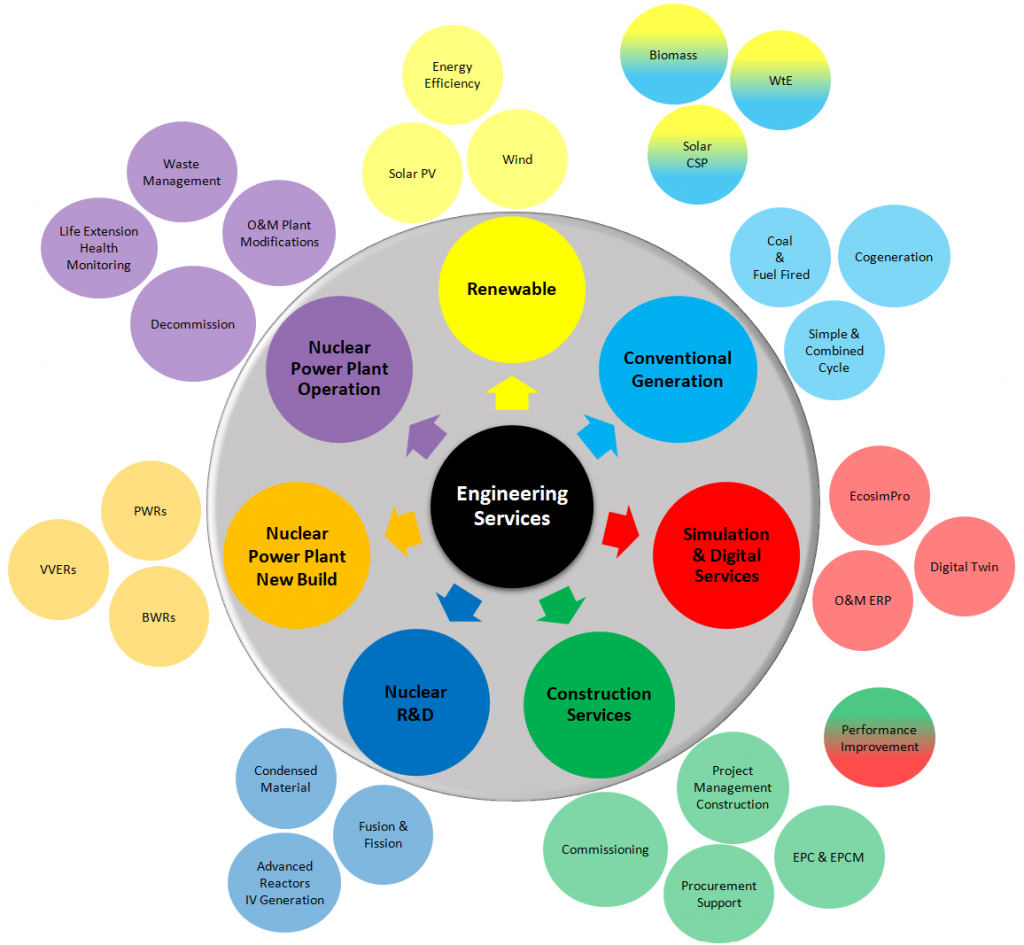
\includegraphics[width=0.8\textwidth]{./object/EAI-proj.png}
    \caption{Domaines couverts par EAI}
\end{figure}

En janvier 2020, EAI à été acquis par China Engineering Group Planning \& Engeneering Co., Ltd. qui appartient à State Owned Assets Supervision and Administration Comission, l'un des plus grand conglomérat d'entreprise mondial.\cite{EAI1}

Ceci fait de EAI une entreprise classifié parmi les 20 premières sociétés internationales en ingénierie et gestion de construction des projets de Génération Électrique (+60 GWe)\cite{EAI1}. Et aussi inclue dans le ranking des 120 plus grandes entreprises internationales d'ingénierie d'après Engineering News-Record.\cite{EAI2}

\subsection{Historique}

L'objectif du groupe Empressarios Agrupados coïncidait avec le lancement du design et de la construction de la centrale nucléaire de Almaraz en Espagne en 1971. Ce projet fut réalisé grâce à l'expérience des entreprises partenaires fondées sur des projets de centrales thermiques conventionnelles, des grandes infrastructures civiles et des station pétrochimiques, et d'une collaboration de l'entreprise américaine Gibbs \& Hill, Inc(GHI).

\begin{wrapfigure}[12]{l}{0.45\textwidth}
    \vspace{-10pt}
    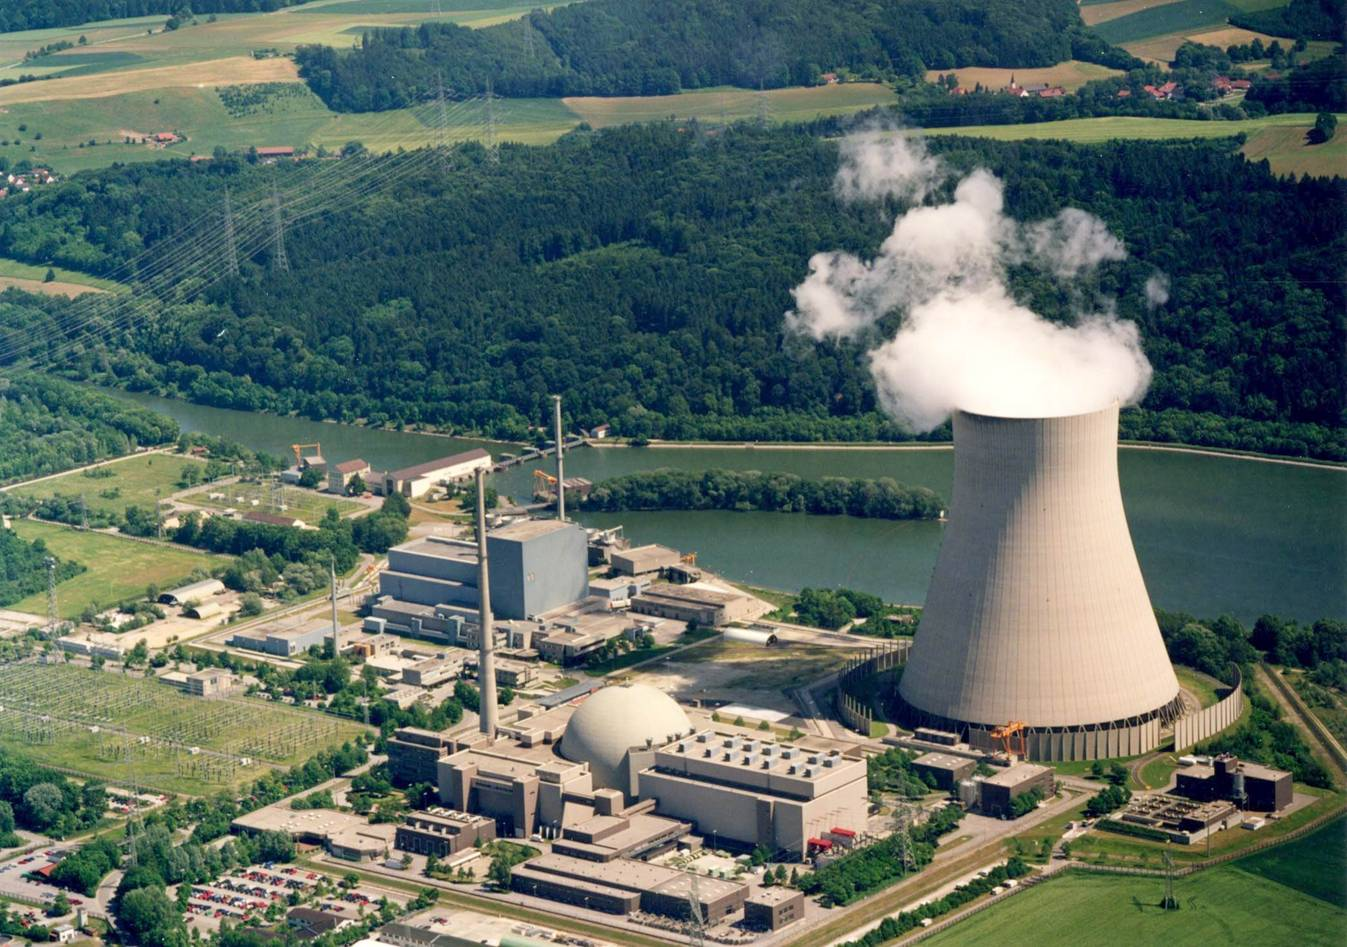
\includegraphics[width=0.75\textwidth]{./object/Almaraz.jpg}
    \caption[caption]{\tabular[t]{@{}l@{}}Centrale Nucléaire \\ Almaraz, Espagne\endtabular}
\end{wrapfigure}

Grâce à cette collaboration, plusieurs autres projets nucléaires furent réalisés en Espagne sur une durée de 10 ans. Ce projet de capacitation technologique à été considéré complété en 1981, grâce à une projet de recrutement dans le domaine d'ingénierie, de design, de la gestion de dépen\-ces et direction de construction. Ceci a alors permit Empressarios Agrupados d'entreprendre le projet de la centrale nucléaire de Trillo sur lequel ont été réalisés plus de 10 million d'heures humaines, avec un personnel d'environ 1400 personnes dont 65\% à titre universitaire.

Cependant avec la paralyzation du programme de construction de centrales nucléaires en Espagne décidée en 1983, Empresarios Agrupados a donc dû se chercher des domaines dans lesquels de diversifier en exploitant ses capacités technologiques existantes. De cette diversification l'entre\-prise à participé dans des projets de centrales thermoélectriques, un programme spatial européen et d'autres projets indépendants.

Avec le programme spatial européen, la stratégie consistait à un société ibérique de l'espace, appelé IberEspacio, qui a été alors fondée en 1987. Les travaux de développement étaient liées sur les lanceurs Ariane 4 et Ariane 5 notamment sur la simulation de systèmes, l'analyse structurelle avancée, la fiabilité, l'analyse des données du vols, et plus. La capacité de développement de ces activités provenaient fondamentalement de l'expertise de l'entreprise dans les domaines du nucléaire.

\begin{wrapfigure}[10]{r}{0.45\textwidth}
    \vspace{-10pt}
    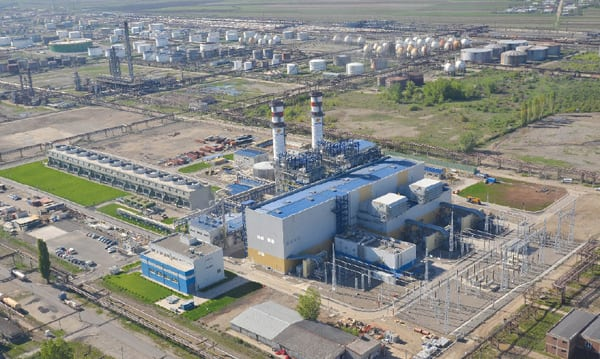
\includegraphics[width=0.75\textwidth]{./object/Brazi.jpg}
    \caption[caption]{\tabular[t]{@{}l@{}}Centrale à Cycle Combiné \\ Brazi, Roumanie\endtabular}
\end{wrapfigure}

Sur les projets thermoélectriques Empresarios Agrupados à réussi à compléter 14 unités à la fin des années 70; 8 en Espagne, 2 au Mexique, 1 au Filipines, 2 au Chile et 1 en Argentine, en plus d'autres travaux de consultation dans ce domaine. Aujourd'hui 31 unités à charbon ont été complétés avec une puissance totale d'environ 17 325MW. % Complete with carbon and Fuel-oil

Au début des années 2000 la génération électrique s'est orienté vers le gaz naturel comme combustible en utilisant des centrales à cycle combiné de haut rendement thermodynamique, et un impacte environmental modéré. C'est donc ainsi que Empresarios Agrupados c'est introduit dans ce domaine en complétant 47 projets avec un puissance conjointe de 28 927MW, 60\% de la puissance étant réalisé sur des projets étrangers.

Empresarios Agrupados participe également à la maintenance des centrales pour la résolution d'incidents, l'adaptation au niveau critère de sécurité, modernisation, surveillance de vieillissement, etc\dots

Elle se maintient désormais à jour sur les avancés technologiques afin d'apporter cet aide sur les centrales en cours de design et pour le reste des centrales en Espagne et à l'étranger. Ceci est possible grâce à la participation dans des projets de recherche et développement, comme le projet ITER, et la collaboration avec des universités et des centres de recherche.

\subsection{Un marché international}

Comme précédemment vu EAI est une entreprise qui opère dans l'ingénierie et la gestion de construction de projets dans le domaine de l'énergie, de l'industrie et de l'infrastructure. Elle a aussi  mené une action agressive, à la fois technologique et commerciale, qui lui a permis de trouver des contrats dans le domaine nucléaire de nombreux pays.

Aux États-Unis elle a réalisé des travaux sur la construction des centrales nucléaires de Comnache Peak 1 et 2, ainsi que pour d'autres services dans les centrales Lasalle, Hope Creek, Haddam Neck et Calverts Cliffs, qui sont actuellement toujours en fonctionnement. À l'autre bout du monde, en Taiwan, EAI à participé dans la construction de la centrale nucléaire de Lungmen sous contrat avec General Electric.

La compagnie porte une présence importante à l'internationale avec des projets en cours dans plus de 40 pays ce qui suscite un marché hautement compétitif et complexe avec de nombreux acteur locaux et internationaux. Cependant EAI a su se démarquer en se spécialisant dans le domaine nucléaire, et en se concentrant sur les projets de grande envergure assurant un travail de qualité, de confiance, et professionnel.

\begin{figure}[ht!]
    \centering
    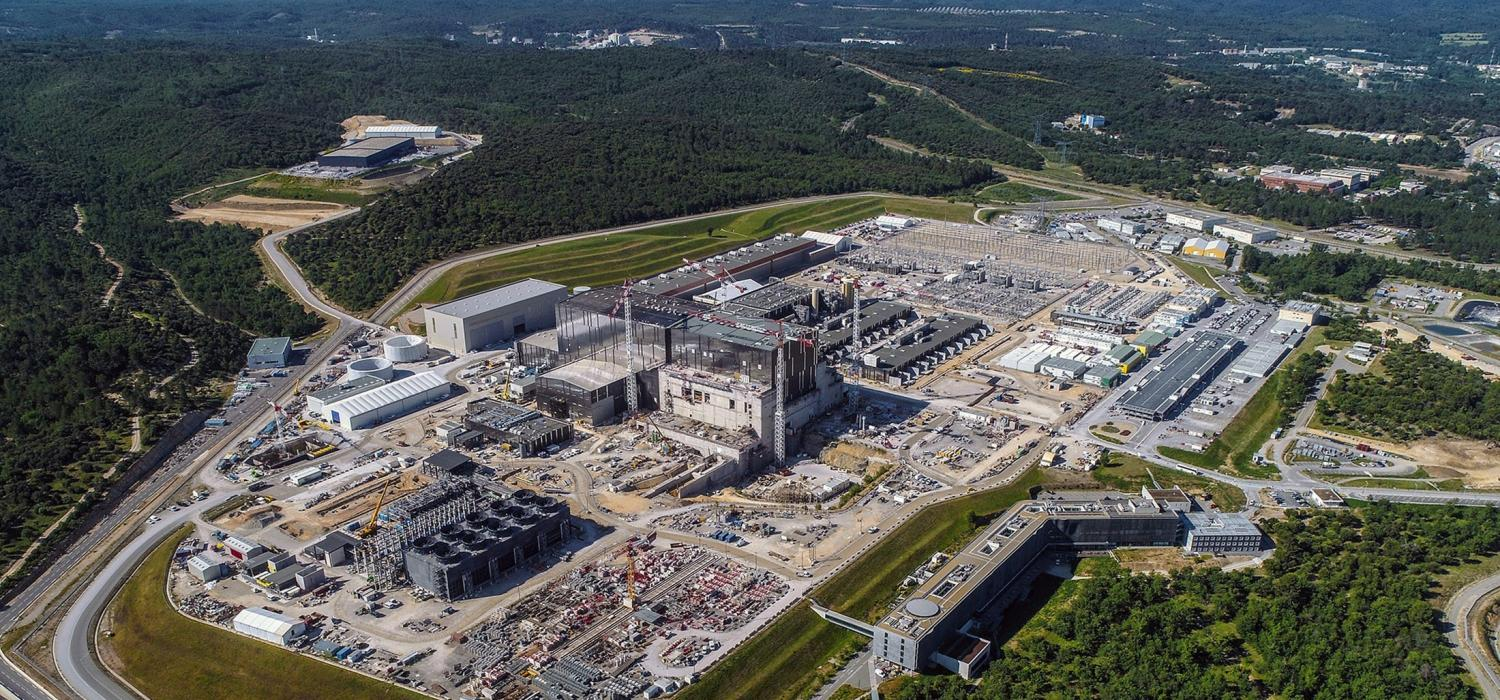
\includegraphics[width=0.6\textwidth]{./object/ITER.jpg}
    \caption{Centrale Nucléaire ITER, France, Cadarache}
\end{figure}

Depuis 16 ans elle fait partie d'un groupe d'entreprise européennes qui ont été sélectionnées pour participer dans le projet ITER, un projet de recherche et développement dans le domaine de la fusion nucléaire. Cependant l'obtention des contrats n'est pas toujours facile, et EAI a dû faire face à des difficultés dans le passé. En 2009 elle a perdu un contrat pour la construction de la centrale nucléaire de Cernavoda en Roumanie, et en 2010 elle a perdu un autre contrat pour la construction de la centrale nucléaire de Belene en Bulgarie.

Ces principaux rivaux avec qui elle fait compétition sont des grandes entreprises internationales, notamment Jacobs Engineering Group Inc., Bechtel Group Inc., Fluor Corporation, et WorleyParsons Ltd.





\subsection{Organisation}

À la tête de EAI se trouve l'équipe de direction exécutive se trouve l'équipe de direction exécutive, comprenant le  directeur général Javier Perea,  le directeur général adjoint F.Javier Goicoechea, le directeur de stratégie Tu Jin et la directrice des finances Dan Zhu, ainsi que d'autres cadres supérieurs. Cette équipe fournit la direction stratégique, supervise et prend les direction majeures de l'entreprise.

La structure de l'entreprise se divise ensuite en deux grandes branches, l'une étant la direction de négoce et l'autre la direction d'ingénieure. À l'intérieur de la direction d'ingénieure s'y retrouve les plusieurs département d'ingénierie; civil, électrique, instrumentation et contrôle, de design, mécanique, et dernièrement de sécurité.

La direction d'ingénierie joue un rôle important dans les opération de l'entreprise. Il est responsable de la conception et du développement des projets nucléaires et infrastructures associés. Le département des design fournit les design civils, électrique, ainsi que le design des centrales, l'ana\-lise des équipements et les systèmes en 3 dimensions.

Ces design sont alors transmis au département qui leur concerne, dans le cas de ce stage, le design des systèmes qu'il a fallut utilisé était fournit au département I\&C et mécanique. Ces design sont mis à jour toute les semaines, certaine fois à cause de problème dans le design, ajout ou modification d'équipements et correction. Les département qui s'appuient dessus doivent donc aussi constamment metre à jour leur travaux à partir de ces changements.

Dans le département I\&C dirigée par mon tuteur Luis Cerrada se trouvent deux branches, l'une étant celle des systèmes de contrôle nucléaire et l'autre celle des systèmes de contrôle conventionnel dirigée par Óscar Petisco qui est aussi le responsable de projet sur ma première mission.

Les ingénieurs du département d'instrumentation est compris d'environ 30 employés dont une dizaine de stagiaires. Ceci vient du fait que l'entreprise accueille beaucoup d'étudiant d'univer\-sité cherchant à valider leur grade, master ou doctorat. Certain continuent alors à travailler dans l'entreprise développant ainsi le début de leur formation professionnelle.

Les ingénieurs dans ce département s'occupent aussi souvent avec plusieurs projets en même temps, la plupart du temps lorsque le travail sur un des projets et mis à jour avec le design fournit, ils alternent avec d'autres. Ceci à aussi été le cas durant mon stage après avoir fini une liste de signaux et passé sur des groupes fonctionnel d'un projet différent.















\newpage

\section{Première mission : Projet Flemalle}

\subsection{Introduction du projet}

En 1951 la centrale à charbon Les Awirs est construite à Flemalle en Belgique, composé de 3 unités avec une production totale de $225\ MW$.\cite{Hist Flemalle} En 1997, après 46 ans de fonctionnement les unités 1,2 et 3 sont arrêtés et démantelé en faveur d'une centrale à biomasse construite en 2005, avec une production de $75\ MW$.\cite{Hist Flemalle2}\cite{Hist Flemalle3} Après 15 ans de fonctionnement, la centrale biomasse est arrêté en 2020, et remplacé par une centrale à gaz à cycle combiné (CCGT), avec une production de $875\ MW$ prévue pour 2025.\cite{Hist Flemalle3}\cite{Hist Flemalle4}



\begin{figure}[ht!]
    \centering
    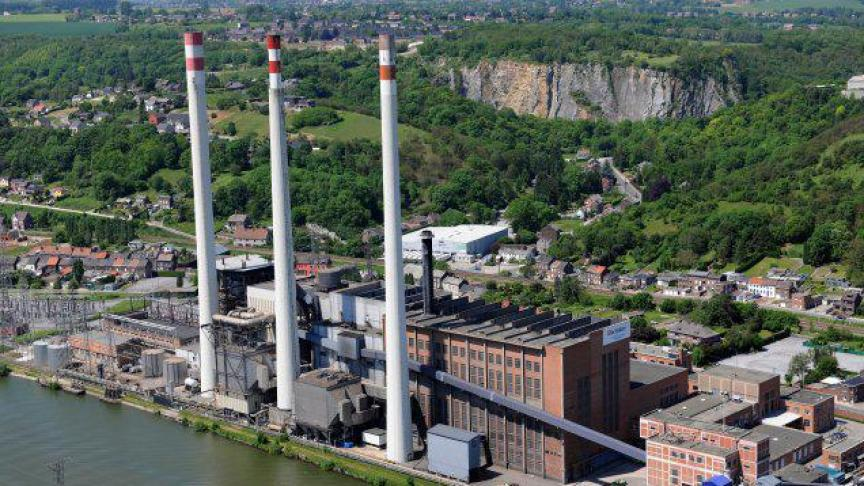
\includegraphics[width=0.6\textwidth]{object/g3-1.jpg}
    \caption{Centrale Les Awirs 11/10/2022}
\end{figure}

Il s'agit d'un projet lancé par Engie, une entreprise française spécialisée dans la production et la fourniture d'énergie. La branche belge est Engie Electrabel, qui est le principal fournisseur d'électricité en Belgique. EAI est un des sous-traitants d'Engie Electrabel pour ce projet et est responsable des systèmes de contrôle-commande de la centrale.


Faisant parti des systèmes de contrôle-commande le DCS est un des systèmes les plus importants de la centrale. Il s'agit d'un système de contrôle distribué, qui permet de contrôler et de surveiller les différents systèmes de la centrale. Il est composé de plusieurs unités de contrôle, chacune responsable d'une partie de la centrale. Le DCS est aussi responsable de la communication avec les autres systèmes de la centrale, comme le système de protection, le système de mesure, et le système de contrôle-commande de niveau supérieur.

Afin d'assurer le bon fonctionnement de la centrale le DCS est relié à plusieurs cartes d'entrées\-sorties qui permettent de communiquer avec les différents capteurs et actionneurs. Ces capteur et actionneurs possèdent chacun des signaux qui leur appartient, c'est pourquoi il est nécessaire de réaliser une liste de signaux pour toutes les cartes d'entrées/sorties. Cette liste de signaux est aussi appelée liste d'entrées/sorties (I/O list).


\subsection{Identification}

La réalisation d'une liste de signaux s'effectue à partir des graphiques P\&ID. Les graphiques P\&ID sont des schémas qui représentent les différents systèmes de la centrale, ainsi que les composants d'instrumentation et de contrôle qui les composent. Ils sont utilisés pour la conception, la construction, et la maintenance des systèmes de la centrale.

On y retrouve tout types d'instrument et d'actionneurs, comme des vannes, des pompes, des capteurs, des transmetteurs, des régulateurs, etc. Chacun de ces composants possèdent des signaux qui leur sont propres, et qui sont utilisés par le DCS pour communiquer avec eux. Il est donc nécessaire de créer une liste de signaux pour chaque carte d'entrées/sorties du DCS.

Dans un premier temps, avant de se lancer sur la liste de signaux, il faut identifier les appareils qui seront câblés au DCS. Pour ceci il faut s'aider du code couleur sur les P\&ID qui mets en évidence les lignes d'instrument en violet. Parmi eux on distingue vite deux types, les capteurs et les actionneurs. Dans la continuité on appellera en général les capteurs des boucles'\footnote{Les capteur en I\&C sont vu comme des capteur à boucle fermé fournissant une rétroaction, d'où le terme boucle} et les actionneurs des équipements de façon à s'adapter à la terminologie utilisé en I\&C


\subsubsection{Boucles}

Parmi les boucles on distingue 3 types différents. Le premier type étant ceux localement accessible sur l'emplacement de l'appareils, notamment les gauges. Il se distingue dans le P\&ID dans une bulle sans trait horizontal. Le deuxième sont ceux qui sont traités un panneau de commande central, il s'agit des boucles dotées d'un transmetteur qui communique directement au DCS, un exemple serai un transmetteur de température. On les identifie par une bulle avec un trait horizontal au milieu. Et Le dernier sont ceux qui sont reliées à un panneau de contrôle local souvent sur un système de contrôle secondaire. On les retrouve par une bulle avec un double trait horizontal au milieu.

\begin{figure}[ht!]
    \centering
    \begin{tikzpicture}
        \foreach \step in {1,2,3} {
                \draw[purple!80!blue!70, thick] (\step*5 - 2,0.5) -- ++ (2,0) arc (90:-90:0.5) -- ++ (-2,0) arc (270:90:0.5);
                \node[purple!80!blue!70] at (\step*5-1,0.25) {ID code};
                \node at (\step*5-1,-0.25) {KKS code};
                \draw[purple!80!blue!70,thick] (\step*5-1,-0.5) -- ++ (0,-0.25);
            }
        \draw[purple!80!blue!70, thick] (7.5,0) -- ++ (3,0);
        \draw[purple!80!blue!70, thick] (12.5,0.05) -- ++ (3,0);
        \draw[purple!80!blue!70, thick] (12.5,-0.05) -- ++ (3,0);

        \node[align=center,scale=0.9] at (4,-1.25) {Traitement Local};
        \node[align=center,scale=0.9] at (9,-1.5) {Traitement sur \\ Panneau de commande \\ Central};
        \node[align=center,scale=0.9] at (14,-1.5) {Traitement sur \\ Panneau de commande \\Local};

    \end{tikzpicture}
    \caption{Différents types de boucles retrouvés sur les P\&ID}
\end{figure}

Dans la liste de signaux nous nous intéresserons uniquement aux instruments reliés au DCS c'est pourquoi on cherchera alors tous les instruments ayant un seul trait violet en vérifiant qu'il s'agisse bien d'un transmetteur dans le cas d'étourdis dans le design des P\&ID.

Pour ceci on peut se référer à l'identification d'instrument (ID code) qui indique le type d'instru\-ment ainsi que ces fonctions. Il s'obtient à partir d'un tableau de correspondance entre le type d'instrument et son ID code. Le tableau figurant ci-dessous :


\begin{table}[ht!]
    \centering
    \resizebox{\textwidth}{!}{
        \begin{tabular}{|c|l|c|c|c|c|}
            \cline{2-6}
            \multicolumn{1}{c|}{} & \multicolumn{5}{c|}{
            \Large{\bfseries{\textsc{Instrument Identification }}}\normalfont\normalsize}                                                                                                                                                                     \\
            \multicolumn{1}{c|}{} & \multicolumn{5}{c|}{\begin{tikzpicture}

                                                                \draw[purple!80!blue!70, thick] (1*5 - 2,0.5) -- ++ (2,0) arc (90:-90:0.5) -- ++ (-2,0) arc (270:90:0.5);
                                                                \node[purple!80!blue!70] at (1*5-1,0.25) {LSCN};
                                                                \node at (1*5-1,-0.25) {XXXXXX XXXXX};
                                                                \draw[purple!80!blue!70,thick] (1*5-1,-0.5) -- ++ (0,-0.25);

                                                                \draw[purple!80!blue!70, thick] (2.5,0) -- ++ (3,0);
                                                                \node at (9.4,0) {\large Functional Identification Code};
                                                                \draw[-latex] (6.5,0) -- ++ (-2,0.25);
                                                            \end{tikzpicture}}                                                                                              \\
            \cline{2-6}
            \multicolumn{1}{c|}{} & \multicolumn{1}{c|}{First Letter}                                                                         & \multicolumn{1}{c|}{Modifier} & \multicolumn{3}{c|}{Succeeding Letters}                                       \\
            \hline
            Letter                & Initiating Variable                                                                                       & Variable Modfifier            & Passive Function                        & Active Function & Function Modifier \\
            \hline
            A                     & Analysis                                                                                                  &                               & Alarm                                   &                 &                   \\
            \hline
            B                     & Burner, Combustion                                                                                        & User's Choice                 & User's Choice                           & User's Choice   & User's Choice     \\
            \hline
            C                     & User's Choice                                                                                             &                               &                                         & Control         & Close             \\
            \hline
            D                     & Density                                                                                                   & Differential                  &                                         &                 &                   \\
            \hline
            E                     & Voltage                                                                                                   &                               & Sensor, Primary Element                 &                 &                   \\
            \hline
            F                     & Flow                                                                                                      & Ratio                         &                                         &                 &                   \\
            \hline
            G                     & User's Choice                                                                                             &                               & Glass, Gauge, Viewing Device            &                 &                   \\
            \hline
            H                     & Hand (Manual Input)                                                                                       &                               &                                         &                 & High              \\
            \hline
            I                     & Current                                                                                                   &                               & Indicate                                &                 &                   \\
            \hline
            J                     & Power                                                                                                     &                               &                                         &                 &                   \\
            \hline
            K                     & Time, Schedule                                                                                            &                               &                                         &                 &                   \\
            \hline
            L                     & Level                                                                                                     &                               & Light                                   &                 & Low               \\
            \hline
            M                     & User's choice                                                                                             &                               &                                         &                 &                   \\
            \hline
            N                     & User's choice                                                                                             &                               & User's choice                           & User's choice   & Trip              \\
            \hline
            O                     & User's Choice                                                                                             &                               & Orifice, Restriction                    &                 & Open              \\
            \hline
            \vdots                & \multicolumn{1}{c|}{\vdots}                                                                               & \vdots                        & \vdots                                  & \vdots          & \vdots            \\
        \end{tabular}}
\end{table}

\newpage

\begin{table}[ht!]
    \centering
    \resizebox{\textwidth}{!}{
        \begin{tabular}{|c|l|c|c|c|c|}
            \multicolumn{1}{c}{\textcolor{white}{Letter}} & \multicolumn{1}{l}{\textcolor{white}{Hand (Manual Input)}} & \multicolumn{1}{c}{\textcolor{white}{Variable Modifier}} & \multicolumn{1}{c}{\textcolor{white}{Glass, Gauge, Viewing Device}} & \multicolumn{1}{c}{\textcolor{white}{Active Function}} & \multicolumn{1}{c}{\textcolor{white}{Function modifier}}
            \\
            \vdots                                        & \multicolumn{1}{c|}{\vdots}                                & \vdots                                                   & \vdots                                                              & \vdots                                                 & \vdots                                                   \\
            \hline
            P                                             & Pressure                                                   &                                                          & Point (Test Connection)                                             &                                                        &                                                          \\
            \hline
            Q                                             & Quantity                                                   & Totalize                                                 &                                                                     &                                                        &                                                          \\
            \hline
            R                                             & Radiation                                                  &                                                          & Record                                                              &                                                        & Run                                                      \\
            \hline
            S                                             & Speed, Frequency                                           & Safety                                                   &                                                                     & Switch                                                 & Stop                                                     \\
            \hline
            T                                             & Temperature                                                &                                                          &                                                                     & Transmit                                               &                                                          \\
            \hline
            U                                             & Multivariable                                              &                                                          & Multifunction                                                       &                                                        &                                                          \\
            \hline
            V                                             & Vibration                                                  &                                                          &                                                                     & Valve, Damper                                          &                                                          \\
            \hline
            W                                             & Weight Force                                               &                                                          & Well, Probe                                                         &                                                        &                                                          \\
            \hline
            X                                             & Unclassified                                               & X | Axis                                                 &                                                                     &                                                        &                                                          \\
            \hline
            Y                                             & Event, State, Presence                                     & Y | Axis                                                 &                                                                     &                                                        &                                                          \\
            \hline
            Z                                             & Position, Dimension                                        & Z | Axis                                                 &                                                                     & Drive, Actuator                                        &                                                          \\
            \hline
        \end{tabular}}
\end{table}

Par exemple, sur ce tableau on peut alors lire qu’une boucle désignée LSCN donne Level-Safety-Control-Trip, ce qui se traduit par un déclencheur de control de niveau de sécurité.

\subsubsection{Équipements}

L'identification des équipements se repose plus sur de la symbologie, car chacun possède un symbole différent pour les différencier. Il se construit à base d'un symbole principal puis des 'accessoires' qui viennent s'ajouter à celui-ci pour apporter plus d'information sur l'appareil. Afin d'éviter une liste exhaustive\footnote{EAI fournit une liste plus complète de symboles auquel il faudra consulter pour les équipements plus étranges.}, ci-dessous sont les principaux équipements rencontrés lors de la réalisation de la liste de signaux.

\begin{figure}[ht!]
    \centering
    \begin{tikzpicture}

        \node at (6,1.5) {\ul{Équipement:}};

        \begin{scope}
            \draw[purple!80!blue!70] (0,0) -- ++ (0.4,0.2) -- ++ (0,-0.4) -- ++ (-0.8,0.4) -- ++ (0,-0.4) -- ++ (0.4,0.2) -- ++ (0,0.5) ++ (0,0.25) circle (0.25cm);
            \node[scale=0.8, color=purple!80!blue!70] at (0,0.75) {M};
            \node at (0,-1) {Vanne Motorisée};
        \end{scope}
        \begin{scope}[xshift=4cm]
            \draw[purple!80!blue!70] (0,0) -- ++ (0.4,0.2) -- ++ (0,-0.4) -- ++ (-0.8,0.4) -- ++ (0,-0.4) -- ++ (0.4,0.2) -- ++ (0,0.5) -- ++ (0.25,0) arc (20:160:0.25) -- ++ (0.25,0);
            \node at (0,-1) {Vanne Pneumatique};
        \end{scope}
        \begin{scope}[xshift=8cm]
            \draw[] (0,0.3) circle (0.5cm) ++ (0.5,0) -- ++ (-0.5,0.5) -- ++ (-0.5,-0.5);
            \node at (0,-1) {Pompe Générale};
        \end{scope}
        \begin{scope}[xshift=12cm]
            \coordinate (Center) at (0,0);
            \draw (Center) -- ++ (0,-0.6) -- ++ (0.25,0) -- ++ (0,1) -- ++ (0.05,0) -- ++ (0,0.1) -- ++ (-0.05,0.25) -- ++ (0,0.5) -- ++ (-0.5,0) -- ++ (0,-0.5) -- ++ (-0.05,-0.25) -- ++ (0,-0.1) -- ++ (0.05,0) -- ++ (0,-1) -- ++ (0.25,0) ++ (0,0.6) -- ++ (0.2,0) -- ++ (0,0.4) -- ++ (-0.4,0) -- ++ (0,-0.4) -- ++ (0.2,0);
            \draw (Center) ++ (-0.25,0.4) -- ++ (0.05,0) ++ (0.4,0) -- ++ (0.05,0);
            \draw (Center) ++ (-0.3,0.5) -- ++ (0.6,0);
            \draw[thick] (Center) ++ (-0.3,0.75) -- ++ (0.6,0) ++ (0,0.5) -- ++ (-0.6,0);
            \draw (Center) ++ (0.03,0.4) -- ++ (0,-0.35) ++ (-0.06,0) -- ++ (0,0.35);
            \draw (Center) ++ (-0.1,0) -- ++ (0,0.05) -- ++ (0.2,0) -- ++ (0,-0.05);
            \node at (0,-1) {Pompe Verticale};
        \end{scope}

        \node at (6,-2) {\ul{Accessoires:}};

        \begin{scope}[yshift=-3cm, xshift=0cm]
            \draw[purple!80!blue!70] (0,0) -- ++ (0.4,0.2) -- ++ (0,-0.4) -- ++ (-0.8,0.4) -- ++ (0,-0.4) -- ++ (0.4,0.2) -- ++ (0,0.5) ++ (0.15,-0.1) -- ++ (-0.15,-0.2) -- ++ (-0.15,0.2);
            \node at (0,-1) {Fail Close};
        \end{scope}
        \begin{scope}[yshift=-3cm, xshift=4cm]
            \draw[purple!80!blue!70] (0,0) -- ++ (0.4,0.2) -- ++ (0,-0.4) -- ++ (-0.8,0.4) -- ++ (0,-0.4) -- ++ (0.4,0.2) -- ++ (0,0.5) ++ (0.15,-0.3) -- ++ (-0.15,0.2) -- ++ (-0.15,-0.2);
            \node at (0,-1) {Fail Open};
        \end{scope}
        \begin{scope}[yshift=-3cm, xshift=8cm]
            \draw[purple!80!blue!70] (0,0) -- ++ (0.4,0.2) -- ++ (0,-0.4) -- ++ (-0.8,0.4) -- ++ (0,-0.4) -- ++ (0.4,0.2) ++ (0,0.5) -- ++ (0,-0.25) -- ++ (0.2,-0.15) ++ (-0.4,0) -- ++ (0.2,0.15);
            \node[align=center] at (0,-1) {Avec caractéristique\\ de contrôle};
        \end{scope}
        \begin{scope}[yshift=-3cm, xshift=12cm]
            \coordinate (center) at (0,0);
            \draw[purple!80!blue!70] (center) ++ (-0.4,0.2) rectangle ++ (0.8,-0.4) -- ++ (-0.8,0.4);
            \filldraw[color=purple!80!blue!70, fill=white] (center) circle (0.1);
            \node at (0,-1) {Vanne Papillon};
        \end{scope}
    \end{tikzpicture}
    \caption{Exemple d'équipements et d'accessoires}
\end{figure}


Parfois on retrouve ces équipements en bleu, ce qui indique que le fonctionnement de l'appareil est à usage manuel. D'autres fois il est contenu dans un cadre pointillé rectangle, ceci montre qu'il s'agit d'appareils qui sont fourni par un fournisseur externe. Dans ces deux cas il n'est pas nécessaire d'ajouter l'équipements dans la liste de signaux. Le premier car l'appareil est donc pas câblé au DCS, et le second car les signaux seront fourni par le fournisseur.

Pour les pompes il faudra se référer à une liste de charge électrique sur laquelle figure la puissance de la pompe ce qui nous permettra ensuite de les classifier selon leur puissance consommée. Par exemple une pompe de plus de $250\ kW$ seront de type M-2\footnote{Moteur de puissance moyenne} et posséderont des signaux en plus notamment un arrêt d'urgence et une mesure de courant. D'autres pompes comme les M-3\footnote{Moteur de puissance élevée avec variateur} possèdent en plus une mesure de vibration et des commandes de position.

\newpage

\subsubsection{Code KKS}

Avec les boucles et équipements vu précédemment il est désormais possible de faire l'identifica\-tion des équipements aui sont câblées au DCS sur les P\&IDs. Ci-dessous un exemple, contenant une vanne hydraulique :



%P&ID example
\begin{figure}[ht!]
    \centering
    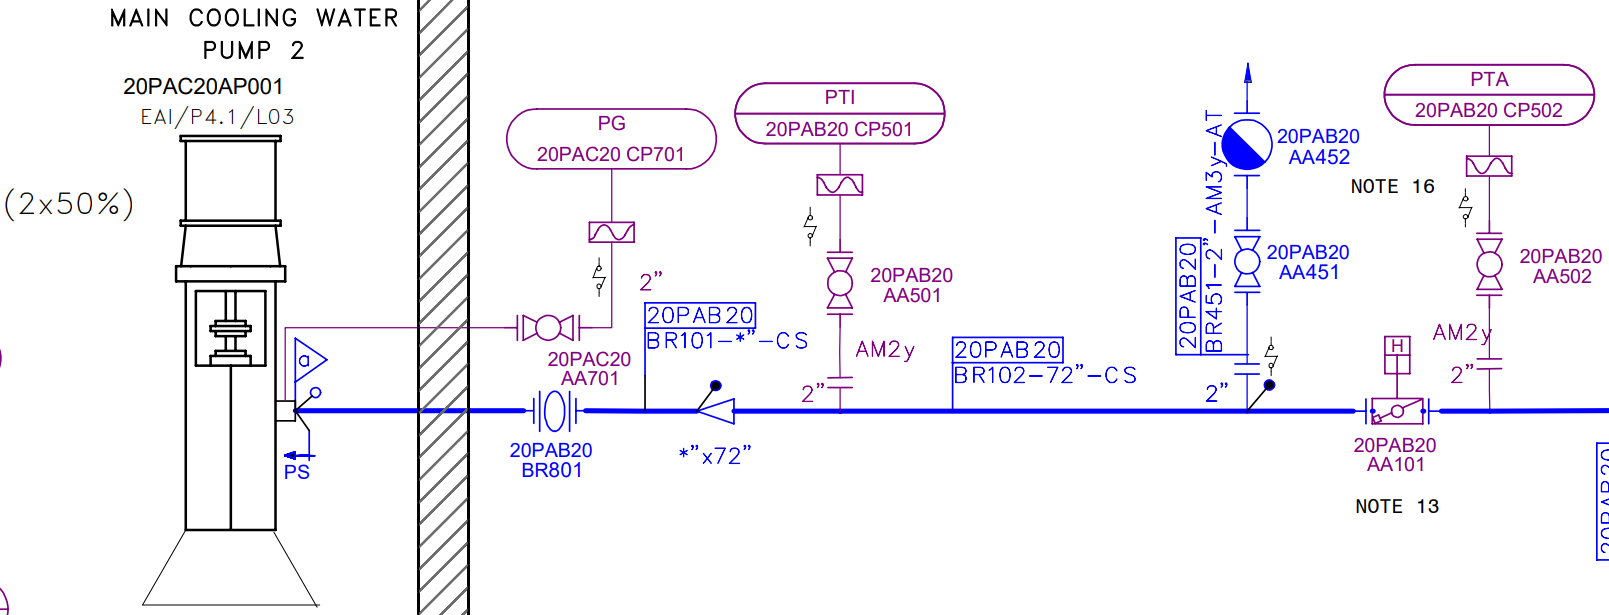
\includegraphics[width=\textwidth]{./object/PID.png}
    \caption{Morceau de P\&ID d'une pompe à eau de refroidissement}
    \label{fig:PID}
\end{figure}

Cependant on remarque que tous les appareils sur le P\&ID viennent avec un code alpha-numér\-ique. Afin de différencier les appareils des uns des autres, tous tiennent un code KKS (Kraftwerk-Kennziechen-System) ou PIS en anglais (Plant Identification System). Celui-ci se décompose en trois parties pour chaque signal. La première partie est le code de l'équipement ainsi que la ligne ou se situe l'appareil, appelé $1^{\text{er}}$ KKS. Le $2^{\text{e}}$ KKS indique le type d'appareil suivi par son numéro sur la ligne. Enfin le $3^{\text{e}}$ KKS donne l'identification du signal câblée au DCS ainsi que le type de signal. Des exemples ci-dessous :


% KKS example
\begin{figure}[ht!]
    \centering
    \begin{tikzpicture}
        \begin{scope}[xshift=-7.5cm]
            \node at (0,0.5) {$\text{\ul{20KGB10}}\ \text{\ul{AP001}}\ \text{\ul{XB01}}$};

            \node at (0.4,1) {$2^{\text{e}}$};
            \draw[thin] (0.4,0.05) -- (0.4,0.35);
            \node at (0.4,-0.25) {Pompe 1};

            \node at (1.35,1) {$3^{\text{e}}$};
            \draw[thin] (1.35,0.35) -- ++ (0.15,-0.15) -- (2.75,0.2) -- ++ (0.15,-0.15);
            \node at (2.75,-0.25) {| Entrée Digitale 01};

            \node at (-1,1) {$1^{\text{er}}$};
            \draw[thin] (-2.85,0.05) -- (-2.7,0.2) -- (-1.15,0.2)  -- ++ (0.15,0.15);
            \node at (-2.85,-0.25) {Équipement 20KGB Ligne 10 |};

            \node at (0,-1.5) {$\text{\ul{20KGB10}}\ \text{\ul{AP002}}\ \text{\ul{YQ01}}$};

            \node at (0.4,-1) {$2^{\text{e}}$};
            \draw[thin] (0.4,-1.95) -- (0.4,-1.65);
            \node at (0.4,-2.25) {Pompe 2};

            \node at (1.35,-1) {$3^{\text{e}}$};
            \draw[thin] (1.35,-1.7) -- ++ (0.15,-0.15) -- (3,-1.85) -- ++ (0.15,-0.15);
            \node at (3,-2.25) {| Sortie Analogique 01};

            \node at (-1,-1) {$1^{\text{er}}$};
            \draw[thin] (-1.15,-1.65) -- ++ (-0.15,-0.15) -- (-2.85,-1.8) -- ++ (-0.15,-0.15);
            \node at (-2.85,-2.25) {Équipement 20KGB Ligne 10 |};
        \end{scope}

        %\draw (-2.5,-3) rectangle (3,1);
        \draw (-1.25,-1) -- ++ (-0.25,-0.15) -- ++ (-1,0) -- ++ (0,0.3) -- ++ (1,0) -- ++ (0.25,-0.15);
        \node[scale=0.75] at (-1.825,-0.25) {20KGB10};
        \draw[thin] (-1.2,-1) -- ++ (0,1) rectangle ++ (-1.25,-0.45);
        \draw (-1.25,-1) -- ++ (0.75,0);
        \draw (0,-1) circle (0.5);
        \draw (0.5,-1) -- ++ (0.75,0);
        \draw (1.75,-1) circle (0.5);
        \draw (2.25,-1) -- (3,-1);
        \draw (1.75,-0.5) -- (2.25,-1) -- (1.75,-1.5);
        \draw (0,-0.5) -- (0.5,-1) -- (0,-1.5);

        \node[align=center, minimum size=1.5cm] at (0,0) {\small General\\\small Pump 1};

        \node[align=center, minimum size=1.5cm] at (1.75,0) {\small General\\\small Pump 2};

        \node at (0,-1.8) {\footnotesize 20KGB10};
        \node at (0,-2.2) {\footnotesize AP001};
        \node at (1.75,-1.8) {\footnotesize 20KGB10};
        \node at (1.75,-2.2) {\footnotesize AP002};
    \end{tikzpicture}
    \caption{Nomenclature de KKS de signaux d'un exemple de deux pompes en série}
    \label{fig:KKS}
\end{figure}


Dans les P\&ID le KKS des signaux n'apparait pas, on ne garde que le $1^{\text{er}}$ et $2^{\text{e}}$ KKS de l'appareil. C'est pourquoi dans le morceau de P\&ID[Figure 3.4] on ne retrouve que le 20PAC20AP001 comme KKS de la pompe. Le $3^{\text{e}}$ KKS sera utilisé pour identifier les signaux dans la liste de signaux et dans les diagrammes logiques de contrôle.

On retrouve souvent sur les boucles des KKS ayant un caractère alphabétique (A,B,C...) en plus au $2^{\text{e}}$ KKS, celui-ci indique une redondance sur la ligne et montre que l'appareil devra être câblée sur une carte E/S différente à son voisin pour éviter que ces derniers arrêtent de fonctionner en cas de panne d'une des cartes E/S

\subsubsection{Signaux de contrôle}

Chaque appareil aillant leurs propres signaux respectifs il est nécessaire de se reposer sur la documentation de ces appareils. Il s'agit de la Control Signal Interface Principle (CSIP) sur lequel on y retrouve les signaux des différents types d'équipement. Chaque moteur, chaque vanne, chaque actionneur câblé au DCS y est présent. Il est donc nécessaire de se référer au CSIP pour attribuer les bons signaux aux appareils [\hyperref[fig:CSIP]{Figure \ref{fig:CSIP}}].

Dans l'exemple d'une vanne motorisé avec signal de position rétroactif, on s'attend à retrouver les signaux de Commande de Fermeture/d'Ouverture, des signaux rétroactif Ouvert/Fermé et de position. Ainsi un exemple the CSIP adapté à cette vanne est présenté ci-dessous :


% CSIP figure example 
\begin{figure}[ht!]
    \centering
    \begin{tikzpicture}
        \begin{scope}[xshift=8cm]
            \draw[thick] (-1,3) rectangle (1,-4);
            \node at (0,2.5) {\textbf{DCS}};
            \foreach \step in {1,2} {
                    \draw[thin] (0.15,2.75-\step) -- ++ (-0.3,0) (0,2.75-\step) -- ++ (0,-0.1) -- ++ (-3,0) -- ++ (0,-0.1) ++ (-0.075,0) -- ++ (0.075,-0.2) -- ++ (0,-0.1) -- ++ (3,0);
                    \node[scale=0.5] at (0,2.9-\step) {$+24$ VDC};

                    \draw[thin] (0.15,1-\step*1.25) -- ++ (-0.3,0) (0,1-\step*1.25) -- ++ (0,-0.1) ++ (-0.075,0) -- ++ (0.075,-0.2) -- ++ (0,-0.1) -- ++ (-3,0) -- ++ (0,-0.1) ++ (0.1,0) -- ++ (-0.2,-0.2) ++ (0.1,0) -- ++ (0,-0.1) -- ++ (3,0);
                    \draw[thin] (-3.25,0.5-\step*1.25) rectangle ++ (0.5,-0.2);
                    \node[scale=0.5] at (0,1.15-\step*1.25) {$+24$ VDC};
                }
            \draw[thin] (0.15,-2.8) -- ++ (-0.3,0) ++ (0.15,0) -- ++ (0,-0.1) -- ++ (-3,0) -- ++ (0,-0.1) ++ (0,-0.3) -- ++ (0,-0.1) -- ++ (3,0) -- ++ (0,-0.1) ++ (0,-0.2) -- ++ (0,-0.1) ++ (0.1,0) -- ++ (-0.2,0);
            \node[scale=0.5] at (0,-2.65) {$+24$ VDC};

            \draw[thin] (-3.25,-3) rectangle ++ (0.5,-0.3);
            \draw[thin] (0.05,-3.5) rectangle ++ (-0.1,-0.2);
            \node[scale=0.6] at (-3,-3.15) {\textbf{ZT}};
            \node[scale=0.45] at (-3.4,-2.9) {$4$-$20$ $m$A};

            \node[scale=0.75] at (2.25,0.5) {VALVE CLOSE};
            \node[scale=0.75] at (2.25,1.5) {VALVE OPEN};
            \node[scale=0.75,align=center] at (2.25,-0.85) {OPEN\\COMMAND};
            \node[scale=0.75,align=center] at (2.25,-2.10) {CLOSE\\COMMAND};
            \node[scale=0.75,align=center] at (2.25,-3.15) {VALVE\\POSITION};

            \node[scale=0.75] at (3.75,1.5) {(XB$01$)};
            \node[scale=0.75] at (3.75,0.5) {(XB$02$)};
            \node[scale=0.75] at (3.75,-0.85) {(YB$11$)};
            \node[scale=0.75] at (3.75,-2.1) {(YB$12$)};
            \node[scale=0.75] at (3.75,-3.15) {(XQ$01$)};
        \end{scope}

        \begin{scope}[xshift=5cm]
            \draw[thick] (-1,3) rectangle (1,-4);
            \node[scale=0.9] at (0,2.5) {\textbf{MOV}};
            \node[scale=0.9] at (0,2.2) {\textbf{ACTUATOR}};
        \end{scope}

        \begin{scope}[xshift=2cm]
            \draw[thin] (-1,3) -- ++ (2,0) ++ (-1,0) -- ++ (0,-0.75) ++ (-0.15,0) -- ++ (0.15,-0.4) -- ++ (0,-3) ++ (0,-0.5) circle (0.5cm) ++ (0,-0.5) -- ++ (0,-1) -- ++ (0.5,0.25) -- ++ (0,-0.5) -- ++ (-1,0.5) -- ++ (0,-0.5) -- ++ (0.5,0.25);
            \node[scale=1.25] at (0,-1.65) {\textbf{M}};
            \foreach \step in {0.1,0.2,0.3} {
                    \draw[thin] (0.15,1.85-\step*2) -- ++ (-0.3,-0.2);
                }
            \draw[thick] (0.03,2.28) -- ++ (-0.06,-0.06) ++ (0,0.06) -- ++ (0.06,-0.06);
            \node[scale=0.6] at (0,3.15) {$400$ VAC 3 Phase};

            \draw[thin,-Latex] (0.7,-3.15) -- ++ (1.25,0);

        \end{scope}

    \end{tikzpicture}
    \caption{CSIP d'une vanne motorisée (MOV) avec signal de position rétroactif câblé au DCS}
    \label{fig:CSIP}
\end{figure}


Le CSIP ne montre de façon simplifiée comment l'équipement communique avec le DCS. Dans la partie logique de la communication avec l'équipement on verra plus tard comment ces signaux sont câblées sur l'actionneur de l'équipement ainsi que les signaux qui seront ensuite transmis par celui-ci directement vers un écran IHM.

\subsubsection{Localisation des cartes E/S}
\label{sec:Localisation}

Le dernier élément qu'il va falloir identifier avant de passer à la création de la liste de signaux est la localisation des cartes E/S. En effet, chaque l'emplacement des cartes E/S est identifiée par un code alphanumérique qui indique sa localisation parmi les différentes zones de la centrale.

Par exemple, sur le projet Flemalle, la centrale se découpe en 4 zones, BOP, WTP, HRSG, et GIS\footnote{Se référer à la liste d'abréviations} qui auront chacun leur propre boîtiers de cartes E/S. Il faudra donc à partir du P\&ID localiser les zones auxquels appartiennent les appareils en s'aidant de leur description et d'une carte de la centrale appelé le Plot Plan. Un exemple évident ci-dessous :


% Plot Plan example
\begin{wrapfigure}[11]{l}{0.5\textwidth}
    \vspace{-15pt}
    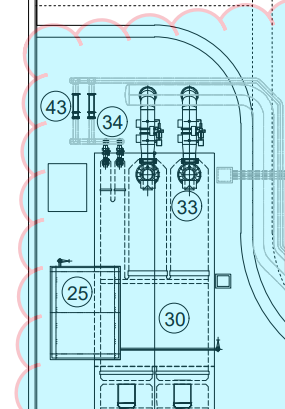
\includegraphics[width=0.4\textwidth]{./object/PlotPlan.png}
    \caption{Morceau du plot plan, zone WTP}
    \label{fig:plotplan}
\end{wrapfigure}
Sur le plot plan on retrouve les 4 zones de la centrale coloriés par des couleurs différentes. Ici la zone du WTP se distingue par une zone bleu.
Dedans on y retrouve les équipements indiqués par des numéros dont le 34 correspondant au Open Cooling Circuit Water Pumps.

Ainsi sur le morceau de P\&ID [\hyperref[fig:PID]{Figure \ref{fig:PID}}] on voit que la pompe 20PAC20AP001 est au numéro 34 situé dans la zone WTP, et que donc les cartes E/S qui lui sont associés seront aussi situés dans la zone WTP.


\subsection{Réalisation de la liste de signaux}

\subsubsection{Logiciel Sigraph}

Pour faciliter la création de cette liste de signaux, EAI utilise un logiciel appelé Sigraph. En plus de pouvoir servir en tant que base de données pour les projets, il contient plusieurs autres fonctionnalités notamment la création de liste de signaux mais aussi la création de diagrammes logiques de contrôle et d'autres documents utiles pour le projet.

Les projets sont tout catégorisés par que le programme appelle des nœud de projet\footnote{En anglais \texttt{Project node}} dans les\-quels on y retrouve les diagrammes logiques, signaux, et autres. À l'intérieur de chaque nœud les systèmes sont répartis chacun par couche structurée contenant leur liste de signaux. Cette liste de signaux est fragmentée en 4 listes dont la liste des boucles et des charges ainsi que leur liste de signaux respectifs.


%fig Sigraph

\begin{figure}[ht!]
    \centering
    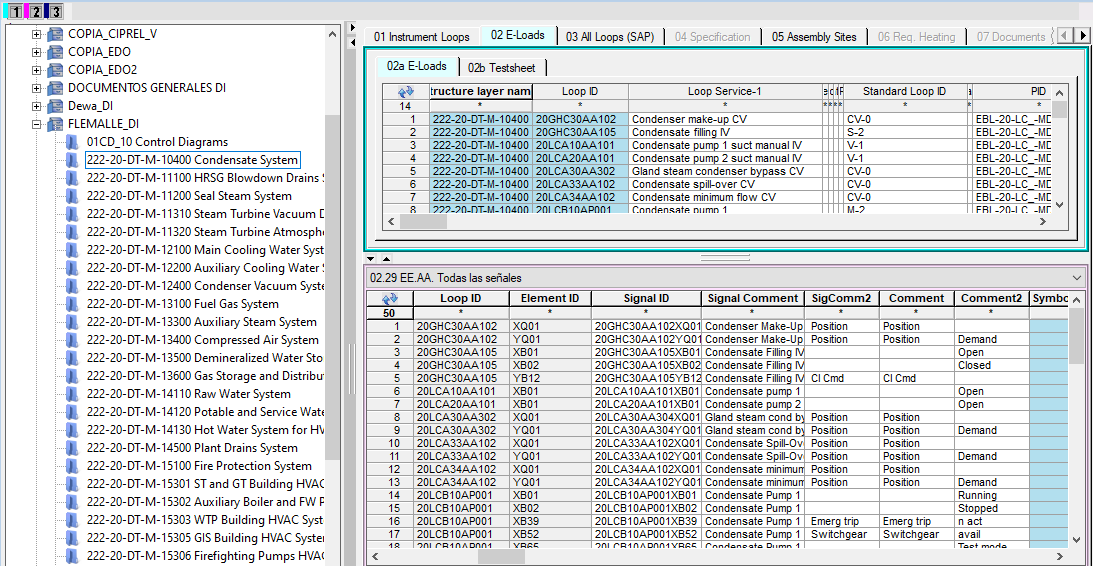
\includegraphics[width=\textwidth]{./object/Sigraph.png}
    \caption{Structure d'un projet sur Sigraph}
    \label{fig:Sigraph}
\end{figure}

Sur cette image on voit bien cette structure dans l'arborescence. Dans le nœud de projet on y retrouve les différents systèmes de la centrale, et dans chaque système on y retrouve les listes. Ci-dessus on peut voir la liste des charges (\texttt{E-Loads}) du système de condensat et la liste de signaux en dessous qui découle de la liste des charges.

On remarque que chaque système possède sa propre identification de document interne le permettant de se différencier des autres systèmes. Mais aussi que les charges sont identifiés par le $1^{\text{er}}$ et $2^{\text{e}}$ KKS de l'appareil et viennent accompagnées d'une description et d'un type d'équipement dans la colonne \texttt{Standard Loop ID}. On remarque aussi da la colonne \texttt{Signal ID} le KKS entier du signal, et les commentaires de signaux à droite qui permet de spécifier dans la liste la fonction du signal.

Comme précédemment évoqué Sigraph permet de fournir la liste de signaux des appareils. Ceci ce fait à travers de la liste de boucle et de charge qui permettent d'identifier l'appareil et lui assigner un type au niveau du \texttt{Standard Loop ID}. L'idée sera donc d'exploiter cette colonne de façon que les appareils d'un certain type reçoivent les signaux correspondant à partir du type qui leur est associé.

Pour ceci il suffit de créer une couche dans laquelle on attribue à chaque type ses signaux respectifs. La liste de charge contiendra la liste de tous les types de charge, et de même avec celle de boucles et ses types de boucle. Pour chacun des types on déclare ensuite les signaux auquel ils devront être câblés dans la partie liste de signaux, et on leur attribue l'identification de matériel dans la colonne \texttt{Loop ID}.

On réalise alors sur Sigraph une liste d'équipements comme ci-dessous, sur lequel on déclare le type dans le \texttt{Loop ID} qui sera référencé lors de l'association des signaux. À côté on précisera aussi la source ainsi que le niveau. Ainsi la liste des de charge sera de la forme :


% Example Sigraph 2
\begin{figure}[ht!]
    \centering
    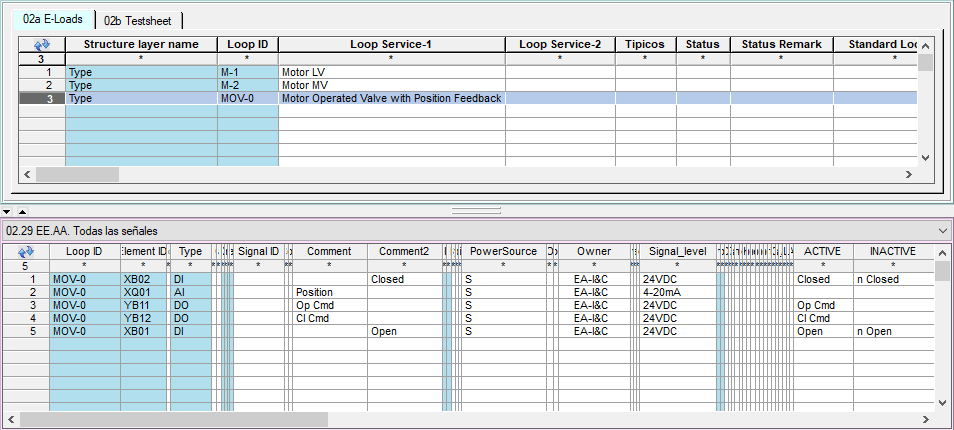
\includegraphics[width=\textwidth]{./object/Sigraph2.png}
    \caption{Exemple de liste de types de charges}
    \label{fig:Sigraph2}
\end{figure}

Pour effectuer ceci il faut s'appuyer sur le CSIP qui contenant les signaux de tous les types d'appareils câblés au DCS. On remarquera que l'exemple ci-dessus reprend le CSIP construit à la \hyperref[fig:CSIP]{Figure \ref{fig:CSIP} } pour définir les signaux propres au MOV avec position rétroactif.

En revenant sur la liste de signaux, on peut donc créer les signaux de chaque type d'appareil. Pour ceci il suffit de sélectionner tous les appareils de la liste et d'appuyer sur un bouton \texttt{Copy Standard Loop}. Comme son nom l'indique il va donc copier les signaux défini dans la liste de types, puis les coller individuellement et respectivement à chaque appareil en utilisant le type précisé dans la colonne \texttt{Standard Loop ID}. Ainsi, lors de la création de la liste de signaux des appareils, Sigraph pourra directement donner la liste de signaux qui découle de la liste des boucles et des charges.

Si on s'imagine que l'on ajoute une \texttt{MOV-0} en série à la suite des deux pompes vu dans l'exemple de KKS [\hyperref[fig:KKS]{Figure \ref{fig:KKS}}] avec un KKS: 20KGB10AA001\footnote{Pour les vannes le KKS de $2^{\text{e}}$ niveau contient AA, au lieu de AP utilisé pour désigner les pompes} on peut alors s'imaginer une liste de signaux qui ressemblera à ceci:


\begin{table}[ht!]
    \centering
    \resizebox{\textwidth}{!}{
        \begin{tabular}{|l|l|c|l|c|c|c|c|}
            \multicolumn{8}{c}{ IO List}                                                                                                                                               \\
            \hline
            Pointname                    & Field Device                & $3^{\text{rd}}$ KKS & Description                            & Active    & Inactive  & Signal Level  & Type   \\
            \hline
            20KGB10AA001XB01             & 20KGB10AA001                & XB01                & General Pumps Discharge  Opened        & Opened    & n Opened  & $24$ VDC      & DI     \\
            \hline
            20KGB10AA001XB02             & 20KGB10AA001                & XB02                & General Pumps Discharge  Closed        & Closed    & n Closed  & $24$ VDC      & DI     \\
            \hline
            20KGB10AA001YB11             & 20KGB10AA001                & YB11                & General Pumps Discharge  Open Command  & Op Cmd    & -         & $24$ VDC      & D0     \\
            \hline
            20KGB10AA001YB12             & 20KGB10AA001                & YB12                & General Pumps Discharge  Close Command & Cl Cmd    & -         & $24$ VDC      & D0     \\
            \hline
            20KGB10AA001XQ01             & 20KGB10AA001                & XQ01                & General Pumps Discharge Position       & -         & -         & $4$-$20$ $m$A & AI     \\
            \hline
            20KGB10AP001XB01             & 20KGB10AP001                & XB01                & General Pump 1  Runnning               & Running   & n Running & $24$ VDC      & DI     \\
            \hline
            20KGB10AP001XB02             & 20KGB10AP001                & XB02                & General Pump 1  Stopped                & Stopped   & n Stopped & $24$ VDC      & DI     \\
            \hline
            20KGB10AP001YB11             & 20KGB10AP001                & YB11                & General Pump 1  Start Command          & Start Cmd & -         & $24$ VDC      & D0     \\
            \hline
            20KGB10AP001YB12             & 20KGB10AP001                & YB12                & General Pump 1  Stop Command           & Stop Cmd  & -         & $24$ VDC      & D0     \\
            \hline

            \multicolumn{1}{|c|}{\vdots} & \multicolumn{1}{c|}{\vdots} & \vdots              & \multicolumn{1}{c|}{\vdots}            & \vdots    & \vdots    & \vdots        & \vdots \\
        \end{tabular}}
\end{table}
\newpage
\begin{table}[ht!]
    \centering
    \resizebox{\textwidth}{!}{
        \begin{tabular}{|l|l|c|l|c|c|c|c|}
            \multicolumn{1}{l}{}         & \multicolumn{1}{l}{}        & \multicolumn{1}{c}{\textcolor{white}{$3^{\text{rd}}$ KKS}} & \multicolumn{1}{l}{\textcolor{white}{General Pumps Discharge  Close Command}} & \multicolumn{1}{c}{} & \multicolumn{1}{c}{} & \multicolumn{1}{c}{\textcolor{white}{Signal Level}} & \multicolumn{1}{c}{\textcolor{white}{Type}} \\
            \multicolumn{1}{|c|}{\vdots} & \multicolumn{1}{c|}{\vdots} & \vdots                                                     & \multicolumn{1}{c|}{\vdots}                                                   & \vdots               & \vdots               & \vdots                                              & \vdots                                      \\
            \hline
            20KGB10AP001XB52             & 20KGB10AP001                & XB52                                                       & General Pump 1  Switchgear Avail                                              & Avail                & n Avail              & $24$ VDC                                            & DI                                          \\
            \hline
            20KGB10AP002XB01             & 20KGB10AP002                & XB01                                                       & General Pump 2  Runnning                                                      & Running              & n Running            & $24$ VDC                                            & DI                                          \\
            \hline
            20KGB10AP002XB02             & 20KGB10AP002                & XB02                                                       & General Pump 2  Stopped                                                       & Stopped              & n Stopped            & $24$ VDC                                            & DI                                          \\
            \hline
            20KGB10AP002YB11             & 20KGB10AP002                & YB11                                                       & General Pump 2  Start Command                                                 & Start Cmd            & -                    & $24$ VDC                                            & D0                                          \\
            \hline
            20KGB10AP002YB12             & 20KGB10AP002                & YB12                                                       & General Pump 2  Stop Command                                                  & Stop Cmd             & -                    & $24$ VDC                                            & D0                                          \\
            \hline
            20KGB10AP002XB52             & 20KGB10AP002                & XB52                                                       & General Pump 2  Switchgear Avail                                              & Avail                & n Avail              & $24$ VDC                                            & DI                                          \\
            \hline
        \end{tabular}}
    \label{fig:IOlist}
    \caption{Liste de signaux réduite de la \hyperref[fig:KKS]{Figure \ref{fig:KKS}}}
\end{table}


On retrouve les signaux que l'on a attribué aux vannes motorisées, le KKS, et une description adaptée à chaque signal. Il s'agit bien sûr que d'une version réduite qui montre essentiellement la fonction du logiciel dans la création de la liste de signaux. En effet, la liste de signaux complète contiendra plusieurs autres colonnes demandées par l'entreprise notamment la référence du système logique et la référence du processus graphique.

\subsubsection{Colonnes supplémentaires post Sigraph}

Certaines colonnes ne sont pas présente sur Sigraph et devront donc être rajoutées manuellement après la création de la liste de signaux. Il s'agit de colonnes qui sont demandé par l'entreprise.

Une colonne qui nous a été demandé pour cette liste de signaux était une traduction française des descriptions de signaux ainsi que leur champs \texttt{Active} et \texttt{Inactive}. Il a donc fallu traduire à la main un total de 850 descriptions ce qui suscite aussi un vocabulaire technique précis et fidèle au fonctionnement des appareils.

Il faudra aussi donner les identifications de documents des systèmes logiques et graphiques qui seront utilisés pour la programmation des appareils. Ces identifications de document sont données par l'entreprise et sont donc à rajouter manuellement sous les colonnes \texttt{Logic} et \texttt{HMI Screen}.

En revenant sur la \hyperref[sec:Localisation]{partie \ref{sec:Localisation}}, la liste de signaux doit aussi contenir une colonne \texttt{Location} qui indique la localisation des cartes E/S auxquels les signaux sont câblés.

Il faudra aussi ajouter une autre colonne pour les équipements redondants de façon à ce que ceux-ci puissent être sur des cartes E/S différentes. En reprenant l'exemple de nos pompes en série [\hyperref[fig:KKS]{Figure \ref{fig:KKS}}] on voit que la deuxième pompe est redondante. Dans l'évènement d'un échec sur une carte E/S, il faut que les qu'une des deux pompes puisse encore fonctionner. Pour ceci il faut que les deux pompes soient câblées sur des cartes E/S différentes. Ainsi, si une carte E/S tombe en panne, la pompe pourra continuer à fonctionner sur l'autre carte E/S.

Il faut donc ajouter une colonne \texttt{Partition} qui indique si l'équipement est redondant et doit se câbler sur une carte E/S différente. Dans le cas où il est redondant, il faudra ajouter une lettre de redondance qui permettra de différencier les deux cartes E/S. Dans l'exemple des deux pompes on s'imagine alors la première avec une partition A et la deuxième avec une partition B.

Enfin la dernière colonne à rajouter pour finaliser la création de la liste de signaux s'agit de la colonne \texttt{Precision} qui indique la précision du signal. En effet, les signaux analogiques possèdent leur propre spécification de précision qui est défini par le constructeur de l'appareil. Pour les signaux rétroactifs de position il s'agit d'une valeur en pourcentage qui indique la précision du signal. On choisira alors de prendre une précision au chiffre significatif 0 car l'arrondi à l'unité suffit. Cependant pour des signaux analogiques de température ou de pression, la précision est souvent donnée en nombre de chiffres significatifs. Dans ce cas on prendra la précision de 1.

Pour les transmetteurs de niveau il faudra se référer à la documentation de l'instrument car tous ne sont pas pareil, certains sont des transmetteurs de niveau à ultrason, d'autres à radar. Chacun possède leur propre précision et il faudra donc se référer à la documentation de l'instrument pour connaître la précision du signal. Dans le cas où la documentation n'est pas présente, on prendra une précision de 1.

\subsubsection{Ajout des PLC}

Sur la centrale certain systèmes sont commandés par des PLC ou des panneaux de commande. Ces derniers sont câblés au DCS et sont donc aussi présent dans la liste de signaux. Cependant, les signaux de ces PLC ne sont pas présents dans le CSIP et il faut donc les ajouter manuellement à la liste.

Pour ceci il faut se référer à la documentation de chaque PLC[\hyperref[fig:PLC]{Figure \ref{fig:PLC}}] pour trouver les signaux qui sont câblés au DCS. Cependant celle-ci ne donne que la description du signal. Il faut donc se suivre une cohérence d'association entre les signaux, leurs fonctions, et leurs KKS. Par exemple on remarque que les signaux YB11 et YB12 sont des commandes de démarrage et d'arrêt.
Ainsi si un PLC avait besoin d’un signal de démarrage, on lui associerait le signal YB11. De même pour un signal d'arrêt on lui associera le signal YB12.


\begin{figure}[ht!]
    \centering
    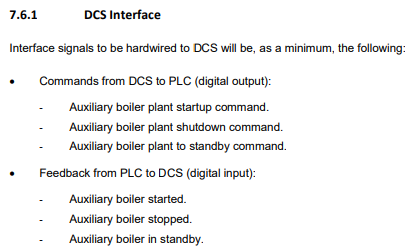
\includegraphics[width=0.7\textwidth]{./object/PLC.png}
    \caption{Morceau de documentation d'un PLC de chaudière auxiliaire}
    \label{fig:PLC}
\end{figure}

Tous les signaux ne sont pas renseignés de cette façon, dans le cas où il faut associer un nouveau signal à un PLC, par exemple pour un signal d'anomalie, il faudra lui attribuer un signal qui se rapproche de sa fonction. Soit les signaux XB31 et XB32 un signal de faille et l'autre d'alarme. Dans la continuité de la logique des signaux XB3- on pourra alors associer le signal XB33 à un signal d'anomalie.

\subsection{Fonctionnement logique}

On a évoqué précédemment les diagrammes logiques qui réalise la communication entre le signal et l'actionneur d'un appareil. Ceci est particulièrement important car les appareils ne portent pas directement les signaux que l'on cherche. Pour ceci il faudra créer des diagrammes logiques qui servent passer un signal et sa fonction au commande propres de l'appareil.

La liste de signaux servira donc de départ pour établir ces diagrammes logiques de contrôle. Cependant il devra aussi contenir l'identification des documents de ces diagrammes pour chaque système dans lequel sera contenu les diagrammes de tous les appareils contenus.

\subsubsection{Diagramme de contrôle logique}

Tous les appareils sur la centrale sont branchés au DCS à partir des cartes E/S. Au niveau du DCS ces appareils sont contrôlés à partir des signaux qui figurent dans la liste de signaux ainsi que d'autres signaux externes venant d'un IHM. Cependant l'actionneur de l'appareil contrôlé possède ses propres entrées et sorties fournit par le constructeur.

Le but est donc à partir des signaux qui proviennent du DCS ou de l'IHM de fournir des commandes à l'actionneur de façon à ce qu'il puisse agir proprement en fonction de ces signaux. Par exemple si l'on souhaite ouvrir une vanne de débordement d'un basin avec les signaux ; \texttt{Basin level switch High High} et \texttt{Valve Closed}, il suffira se brancher ces deux signaux sur un porte \texttt{AND} dont la sortie et branché à la commande d'ouverture sur l'actionneur. Ainsi dès que niveau d'eau commence à être trop haute les signaux provenant du DCS permettent de contrôler directement la vanne en faisant recours à cette logique.

Sur Sigraph cette logique se réalise directement grâce à la liste de signaux présente sur le projet. Dans la hiérarchie de projet on crée un dossier portant l'identifiaction du document des diagrammes logiques du système en question. Dans ce dossier on y retrouve les diagrammes logiques de tous les appareils du système. Chaque diagramme logique est identifié par le KKS de l'appareil auquel il est associé et vient avec une Template dans lequel figure l'actionneur de l'appareil. Cette Template vient directement d'un document interne appelé \texttt{Control Diagrams Macro \& } \texttt{Temp\-late}, couramment appelé la macro.


\begin{figure}[ht!]
    \centering
    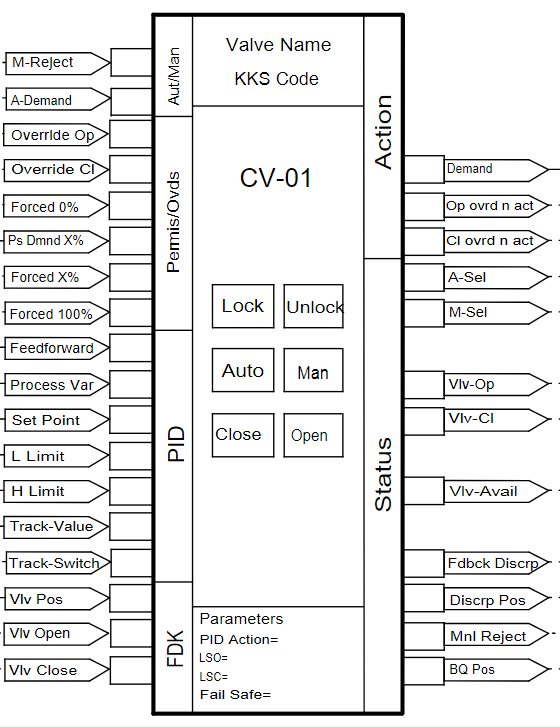
\includegraphics[height=0.6\textwidth]{./object/macro.png}
    \caption{Exemple d'un actionneur une vanne de contrôle contenue dans la macro}
\end{figure}

Sur la macro on y ajoute les signaux qui nous sont besoin pour le fonctionnement de la vanne de contrôles. Ceci peuvent-être des signaux venant des boucles fournissant des donnés sur le niveau, pression, etc\dots. À la suite on y ajoute des portes logiques afin de fournir le rôle cherché à l'actionneur.

À gauche de la macro on y retrouve les signaux d'entrée du DCS qui sont câblés à l'actionneur à travers des cartes E/S, notamment ceux des boucles ou des signaux de l'appareil. À droite on y retrouve les signaux de sortie de l'actionneur qui sont câblés à un écran IHM à travers des variables en mémoire. On contrôle ainsi l'actionneur de soit de façon automatique grâce aux signaux provenant du DCS ou de façon plus manuelle en utilisant l'IHM pour fournir des commandes à l'actionneur.

Après avoir fourni la Template respective à l'appareil associé il faut alors faire la logique de contrôle de l'appareil à partir de la description fonctionnelle de l'appareil.
En utilisant cette description il est alors possible de reprendre les signaux de la liste de signaux et de les brancher sur la Template de façon à ce que l'actionneur de l'appareil puisse être contrôlé par le DCS à travers des portes logiques.


\newpage
\begin{figure}[ht!]
    \centering
    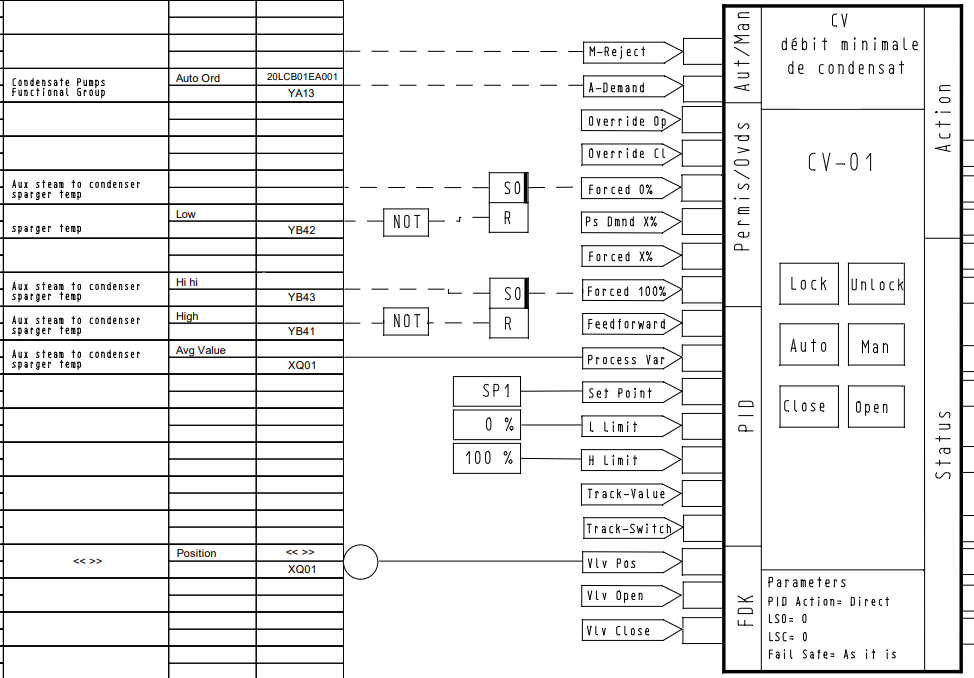
\includegraphics[width=0.7\textwidth]{./object/CV.png}
    \caption{Exemple de logique de contrôle d'une vanne de contrôle}
\end{figure}

On voit donc à partir des portes logique que la vanne ci-présente s'ouvrira de façon forcée si la température de la chaudière dépasse une certaine température \texttt{High High} et à l'inverse se ferme si la température est trop basse \texttt{Low Low}. De plus on remarque qu'un signal de position est également câblée permettant ainsi de connaître la position de la vanne.

\newpage
\section{Autres Missions: Projet North London}

\subsection{Introduction}

En plus de la réalisation de la liste de signaux, j'ai aussi eu l'occasion de travailler sur un autre projet. Il s'agit d'un projet d'une centrale à biomasse à North London. Ce projet est un projet de conception de centrale à biomasse qui sera construite pour le NLWA\footnote{North London Waste Authority}.

Il s'agit du développement d'une centrale de récupération d'énergie (ERF) produisant de l'élec\-tricité à partir de déchets résiduels comme combustible et capable de fournir une puissance électrique d'environ 84 MW.\cite{NLEAI} Elle sera construite à partir de la centrale existante Edmonton EcoPark, qui est une centrale de traitement des déchets ménagers et commerciaux.


\begin{figure}[ht!]
    \centering
    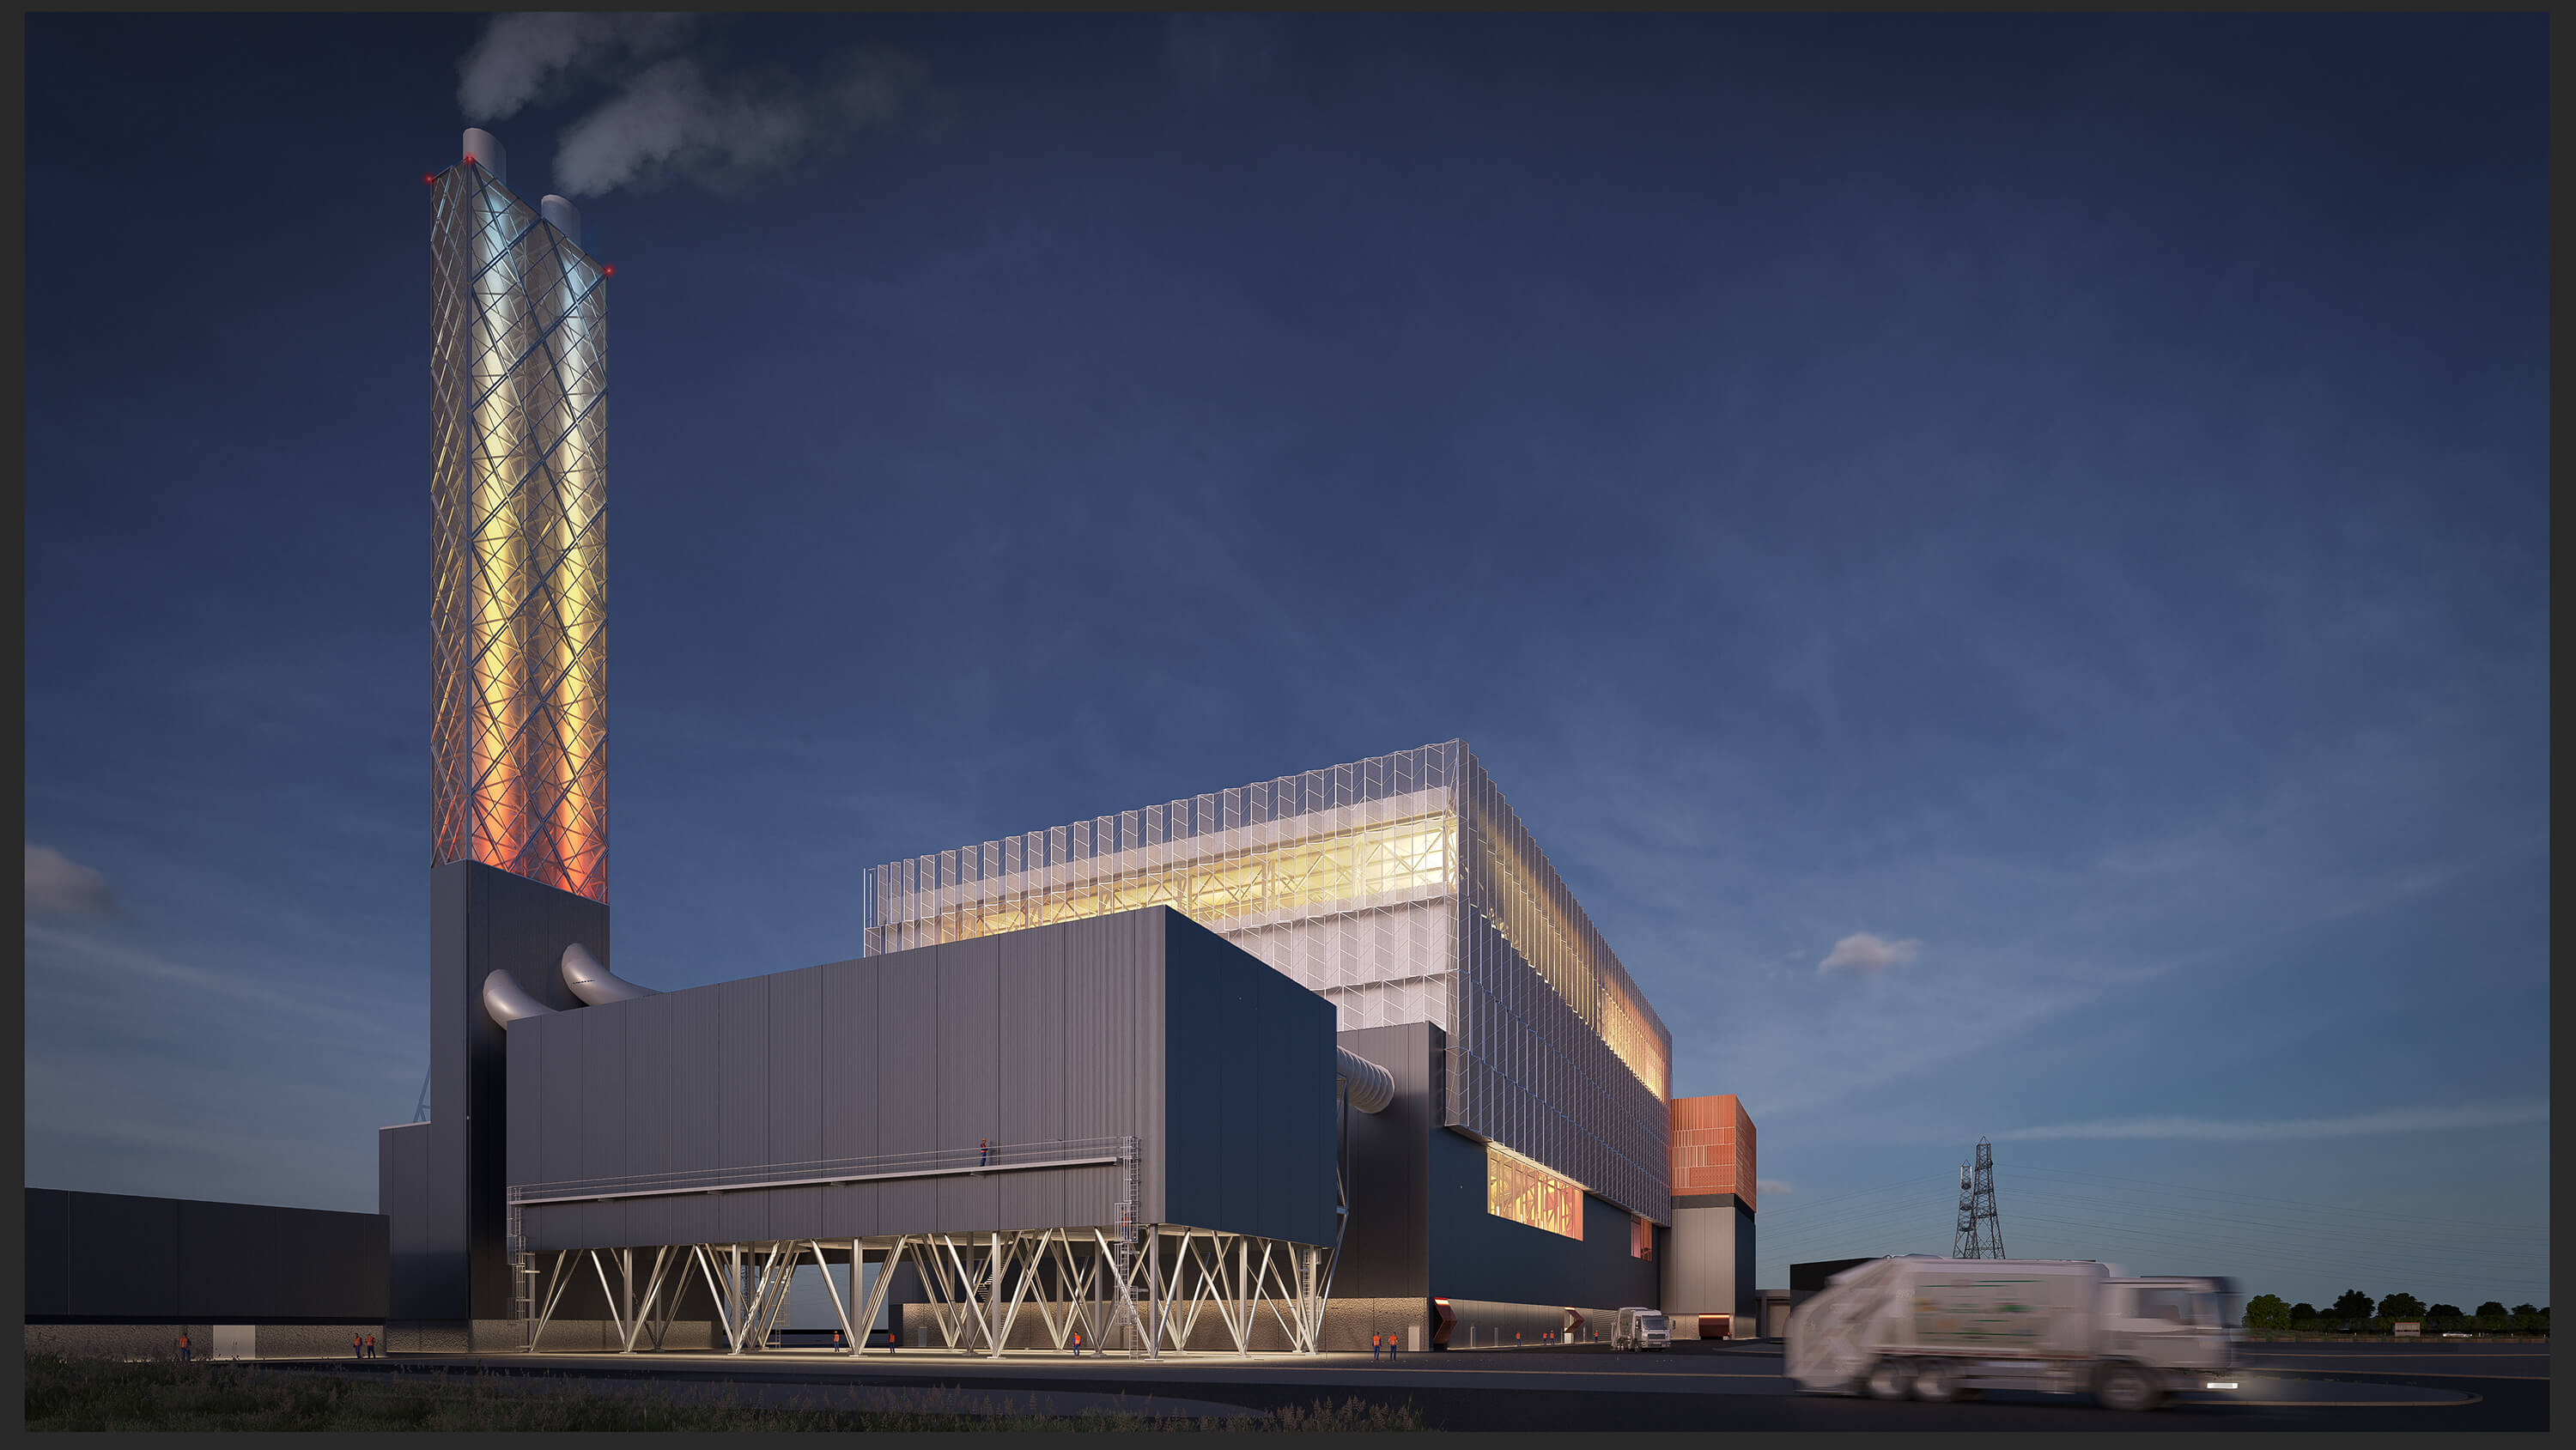
\includegraphics[width=0.6\textwidth]{./object/NLHP.jpg}
    \caption{Centrale de récupération d'énergie de North London}
\end{figure}


Le but de ce projet est d'utilise les déchets de la ville de Londres pour produire de l'électricité. En effet, la ville de Londres produit environ 700 000 tonnes de déchets par an. Depuis 1971 ces déchets sont envoyés dans des décharges ou incinérés ce qui porte un impact néfaste sur l'environ\-nement. Le projet permettra donc de réduire les émissions de gaz à effet de serre de la ville de Londres en utilisant les déchets comme combustible pour produire de l'électricité.

Elle pourra ainsi fournir de l'électricité à environ 127 000 foyers et réduire les émissions de gaz à effet de serre de la ville de Londres de 215 000 tonnes par an. Elle permettra aussi de réduire les déchets envoyés en décharge de 50\% et de recycler 135 000 tonnes de métaux par an.

EAI participe à ce projet en s'occupant de la conception de la centrale et de la partie contrôle-commande. Pour ceci il faudra réaliser la liste de signaux de la centrale ainsi que les diagrammes logiques de contrôle. Cependant mon rôle dans ce projet sera notamment mis à jour la liste de signaux ainsi que de maintenir un système au niveau de ses diagrammes hiérarchique des groupes fonctionnels et descriptions fonctionnelles.

\subsection{Hiérarchie des groupes fonctionnel}

Pour la mise à jour de la liste de signaux il a fallu reprendre le P\&ID du système de vapeur principale, extraction, vapeur auxiliaire et système de dérivation,
et reprendre la liste sur Sigraph afin de l'adapter avec les modification du système. Le gros souci étant que les logiques ont déjà été réalisé à partir des signaux précédents. Il a donc fallu faire attention à ne pas supprimer les appareils qui ont leur logique associée et de remplacer leurs KKS. Il a donc fallu reprendre les étapes de la création de la liste de signaux en reprenant le P\&ID et repérant les appareils qui ont été supprimés, ajoutés ou modifiés.

Cependant, la liste de signaux n'est pas la seule chose à mettre à jour. En effet, il a fallu aussi adapter la hiérarchie des groupes fonctionnels du système. Pour ceci il faut réaliser un diagramme hiérarchique des groupes fonctionnels.

Un diagramme hiérarchique de groupes fonctionnels est une représentation graphique qui illustre les relations et les connexions entre différents groupes fonctionnels dans un. Il met en évidence la structure hiérarchique des groupes fonctionnels en montrant comment ils sont reliés aux appareils de contrôle contribuant à la fonction du groupe. Ce type de diagramme est utilisé pour visualiser et organiser les différentes caractéristiques fonctionnelles du système de manière claire et systématique.

Chaque groupe fonctionnel possède son propre diagramme dans lequel on retrouve le niveau fonctionnel et le niveau des appareils. Dans le niveau des appareils on retrouve les vannes contrôlées par le DCS avec leur KKS et description. On réunit alors les vannes dans leur groupe fonctionnel respectif à partir de leur fonction au niveau du système. Par exemple, si l'on s'imagine une vanne d'isolation d'une chaudière, on la retrouvera dans le groupe fonctionnel de l'échangeur de chaleur.


\begin{figure}[ht!]
    \centering
    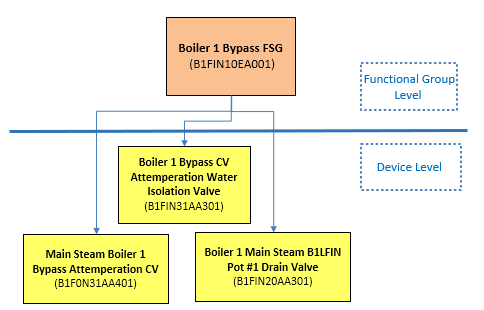
\includegraphics[width=0.6\textwidth]{./object/diag.png}
    \caption{Exemple de diagramme hiérarchique du groupe fonctionnel d'une chaudière}
    \label{fig:diag}
\end{figure}

On voit donc bien sur la figure ci-dessus [\hyperref[fig:diag]{Figure \ref{fig:diag}}] que le groupe fonctionnel de la chaudière est composé de plusieurs vannes qui ont chacune leur propre fonction. Pour ceci il faut donc reprendre le P\&ID du système et repérer les appareils qui ont été ajoutés, supprimés ou modifiés. Il faudra alors les ajouter, supprimer ou modifier dans le diagramme hiérarchique du groupe fonctionnel en veillant à ce que les vannes soient bien dans le groupe fonctionnel qui est indiqué sur les P\&ID.

Ce diagramme hiérarchique est ensuite inclus dans la base de données du projet afin qu'il puisse être mis en commun avec le reste des diagrammes hiérarchique. Il faut donc les ajouter sur Sigraph dans le dossier du système en question, et puis les maintenir au fur et à mesure que le projet avance et que les modifications évoluent.

Pour les appareils et systèmes redondant on distinguera ceci à partir de leur couleur verte. Cette couleur permet d'identifier rapidement les éléments redondants dans le diagramme. En utilisant des couleurs distinctes pour représenter les redondances, il est plus facile de repérer les doublons ou les répétitions d'actions ou de fonctions et donc de se concentrer sur les éléments qui ne sont pas redondant pour la compréhension générale du système.

\newpage
\begin{figure}[ht!]
    \centering
    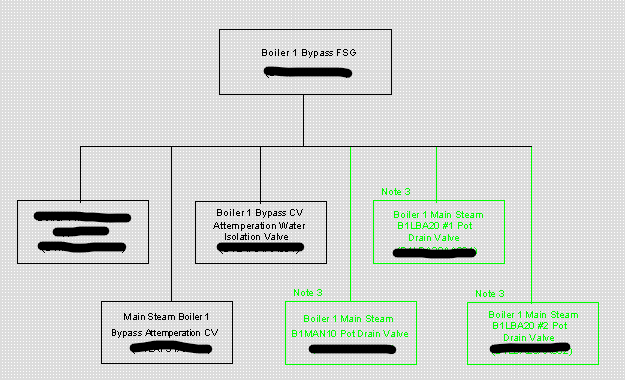
\includegraphics[width=0.6\textwidth]{./object/SigH.png}
    \caption{Exemple de diagramme hiearachique sous Sigraph}
\end{figure}

Ces diagrammes permettent d'obtenir une vue d'ensemble du projet en fragmentant les différents systèmes en fonction des rôles qui leur sont dédiés. Ceci est particulièrement utile car elle permet aussi de voir les relations entre les différents systèmes et de pouvoir les relier entre eux. En effet, les diagrammes hiérarchique des groupes fonctionnels sont aussi utilisés pour réaliser la description fonctionnelle du système.

\subsection{Description Fonctionnelle}

Dans n'importe quel projet d'ingénierie il est important de pouvoir décrire le fonctionnement d'un système. Pour ceci il existe un document appelé la description fonctionnelle du système. Elle fait référence à une explication détaillée ou à une spécification du fonctionnement et du comportement prévus d'un instrument, d'un système ou d'une boucle de contrôle particulière.


\begin{figure}[ht!]
    \centering
    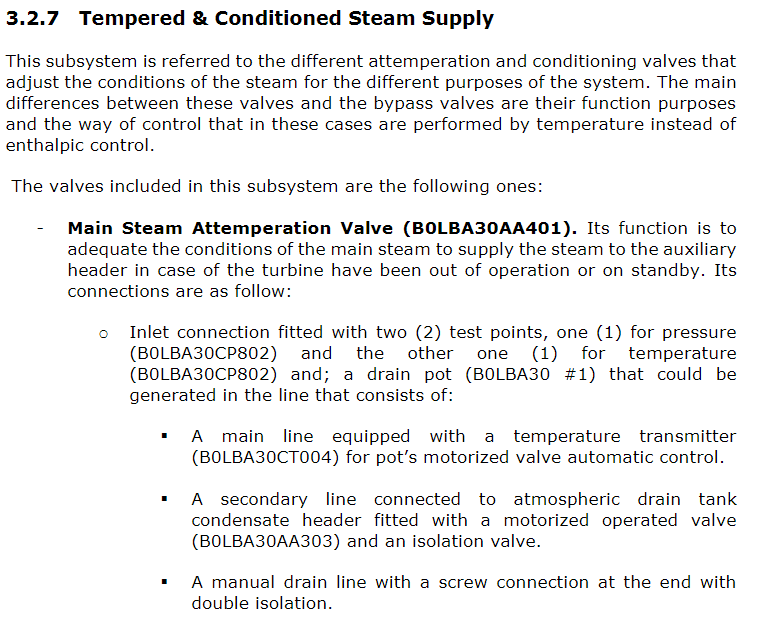
\includegraphics[width=0.6\textwidth]{./object/FD.png }
    \caption{Morceau de description fonctionelle d'une chaudière}
\end{figure}

Une description fonctionnelle décrit le but, les entrées, les sorties et les actions de contrôle de l'instrument ou du système. Elle fournit une compréhension claire de la manière dont l'instrument ou le système doit fonctionner et interagir avec d'autres composants au sein d'un système de contrôle plus vaste. Elle décrit la fonctionnalité souhaitée en termes de variables de processus, de consignes, d'alarmes, de verrouillages, de modes de contrôle et d'autres paramètres pertinents.

La description fonctionnelle sert aussi de plan pour les ingénieurs, les techniciens et les opérateurs impliqués dans la conception, la mise en œuvre et la maintenance du système d'instrumen\-tation et de contrôle. Elle garantit une compréhension commune de la manière dont le système doit fonctionner et facilite la communication et la collaboration efficaces entre les parties prenantes. Elle sert également de référence pour les tests d'acceptation et les audits de sécurité.



Sur le projet North London il a fallu s'appuyer sur des document internes de l'entreprise pour retrouver certaines informations sur le système en question. Notamment sur les pots à condensat qui servent à évacuer le condensat accumulé grâce a des vannes de purge et des transmetteurs de température et de pression

En s'appuyant sur les diagrammes hiérarchique des groupes fonctionnels, et la liste de signaux des divers instruments du système, on peut alors réaliser la description fonctionnelle du système. Il faut préciser leur rôle, leur fonction, leur entrée et leur sortie.




\newpage
\section{Conclusion}

En conclusion ce stage m'a permis de découvrir le monde de l'industrie et de l'ingénierie. Notamment dans un département qui faisait partie de mon projet professionnel et qui m'as permis de me familiariser avec le domaine de l'instrumentation et contrôle. Ceci m’a permis au passage de m'intér\-esser au monde de l'entreprise ainsi que celui d'ingénierie.

J'ai également réussi à compléter les tâches qui m'ont été confié et à m'adapter à la vie en entreprise. Apprenant à travailler en équipe et à communiquer avec mes collègues dans un environnement et un travail de domaine international, faisant l'usage de mes capacités linguistiques.

J'ai découvert comment fonctionne le développement d'un projet et les étapes qui le compose du point de vue des échanges entre départements. J'ai également réussi à assister mes collègues dans leurs tâches et à les aider dans leur travail tout en m'intéressant à la tâche qui m'as été confié.

J'ai su consulter de manière autonome et identifier les informations nécessaires à la réalisation de mes tâches, notamment lors de la réalisation de la liste de signaux ainsi que m'adapter à la dynamique de projet et aux changements qui peuvent survenir.

La liste de signaux m'as aussi permis à pouvoir lire les P\&ID de façon claire et à comprendre le fonctionnement de certains systèmes de contrôle-commande au niveau de leur fonctionnement logique et hiérarchique, ce qui m'as permis d'identifier et corriger des erreurs durant le stage.








%text intro

% functional group + Hierarchie 


































% Table des Figures?
\newpage
\section{Liste des Figures}\lofwithouttitle
\section{Liste des Tables}\lotwithouttitle



\clearpage
\pagestyle{fancy}
\begin{thebibliography}{9}
    \bibitem{RR jobs}
    Communiqué de presse, Rolls-Royce, 11 Novembre 2020,\\ \url{www.rolls-royce.com/media/press-releases/2020/11-11-2020-nuclear-power-stations-will-create-6000-uk-levelling-up-jobs-by-2025.aspx}, \\accédé le 07/05/2023

    \bibitem{Hist Flemalle}
    Communiqué de presse, Engie, 28 Octobre 2020,\\\url{corporate.engie.be/nl/press/release/definitieve-sluiting-van-de-elektriciteitscentrale-van-les-awirs-flemalle-luik}, \\accédé le 16/05/2023

    \bibitem{Hist Flemalle2}
    Article, Argus Media, 3 Septembre 2020,\\\url{www.argusmedia.com/en/news/2138242-engie-closes-belgian-les-awirs-biomass-plant},\\ accédé le 16/05/2023

    \bibitem{Hist Flemalle3}
    Article, BioEnergy, 4 Septembre 2020,\\\url{www.bioenergy-news.com/news/engies-les-awirs-biomass-plant-closes/},\\ accédé le 16/05/2023

    \bibitem{Hist Flemalle4}
    Communiqué de presse, 27 Octobre 2022,\\\url{johncockerill.com/en/press-and-news/news/john-cockerill-will-supply-the-largest-hrsg-and-most-efficient-boilers-in-the-world/}, \\accédé le 16/05/2023

    \bibitem{EAI1}
    Présentation d'entreprise, \\\url{www.empresariosagrupados.es/inicio/presentacion/},\\ accédé le 09/06/2023.

    \bibitem{EAI2}
    Ranking d'entrprise, Engeneering News Record, 2019, \\\url{www.enr.com/toplists/2019-Top-225-International-Design-Firms-2}, \\ accédé le 09/06/2023.

    \bibitem{NLEAI}
    Déscription de projet de la centrale de North London, Empressarios Agrupados \\\url{hwww.empresariosagrupados.es/en/renewable/north-london-heat-power/}, \\accédé le 11/06/2023.

    \bibitem{NLHP}
    Article, \emph{About the North London Heat and Power Project}, NLWA, \\\url{nlwa2.circle-interactive.co.uk/project/about-north-london-heat-and-power-project},\\accédé le 11/06/2023.
\end{thebibliography}

\end{document}